% !TEX root = userguide_jp.tex
%----------------------------------------------------------
\chapter{ファイル仕様}

%----------------------------------------------------------
\section{スタンダードモード用入力ファイル}
\label{Ch:HowToStandard}


スタンダードモード用入力ファイルは次のような格好をしています。

\begin{minipage}{10cm}
\begin{screen}
\begin{verbatim}
W = 2
 L = 4
 model = "spin"
 method = "Lanczos"

 lattice = "triangular lattice"
//mu = 1.0
// t = -1.0
// t' = -0.5
// U = 8.0
//V = 4.0
//V'=2.0
J = -1.0
J'=-0.5
// nelec = 8
2Sz = 0
\end{verbatim}
\end{screen}
\end{minipage}

大まかなルールは次のとおりです。
\begin{itemize}
\item 各行にはひと組ずつキーワード(\verb|=|の前)と
  パラメーター(\verb|=|の後)が書かれており間は\verb|=|で区切られています。
\item 各キーワードは順不同に記述できます。
\item 空白行、または\verb|//|で始まる行(コメントアウト)は読み飛ばされます。
\item 各キーワード、パラメーターの大文字$\cdot$小文字は区別されません。
  ダブルクオート、空白は無視されます。
\item 必ず指定しなければいけないパラメーター、
  指定しない場合デフォルト値が使われるパラメーター、
  (他のパラメーターの組み合わせによっては)使われないパラメーターが存在します。
  使われないパラメーターが指定された場合にはプログラムは終了し、
  入力ファイルをチェックするようにというメッセージが表示されます。
\end{itemize}

次に各キーワードの説明をします。

\subsection{計算の種類に関する必須パラメーター}

\begin{itemize}

\item \verb|model|

{\bf 形式 :} 文字列(\verb|"Fermion Hubbard"|, \verb|"Spin"|, \verb|"Kondo Lattice"|, 
\verb|"Fermion HubbardGC"|, \verb|"SpinGC"|, \verb|"Kondo LatticeGC"|, 
\verb|"SpinGCCMA"|のいずれか)

{\bf 説明 :} 計算対象の模型を指定します。上記の文字列はそれぞれ
カノニカル集団のフェルミ粒子Hubbard模型
\begin{align}
H = - \mu \sum_{i \sigma} c^\dagger_{i \sigma} c_{i \sigma} 
- \sum_{i \neq j \sigma} t_{i j} c^\dagger_{i \sigma} c_{j \sigma} 
+ \sum_{i} U n_{i \uparrow} n_{i \downarrow}
+ \sum_{i \neq j} V_{i j} n_{i} n_{j},
\label{fml4_1_hubbard}
\end{align}
同じくカノニカル集団のスピン模型 ($\{\sigma_1, \sigma_2\}={x, y, z}$)
\begin{align}
H &= -h \sum_{i} S_{i z} - \Gamma \sum_{i} S_{i x} + D \sum_{i} S_{i z} S_{i z}
\nonumber \\
&+ \sum_{i j, \sigma_1}J_{i j \sigma_1} S_{i \sigma_1} S_{j \sigma_1}+ \sum_{i j, \sigma_1 \neq \sigma_2} J_{i j \sigma_1 \sigma_2} S_{i \sigma_1} S_{j \sigma_2} ,
\label{fml4_1_spin}
\end{align}
カノニカル集団の近藤格子模型(Hubbard模型と同様に$U$と$J$を入れることも可能)
\begin{align}
H &= - \mu \sum_{i \sigma} c^\dagger_{i \sigma} c_{i \sigma} 
- t \sum_{\langle i j \rangle \sigma} c^\dagger_{i \sigma} c_{j \sigma} 
+ \frac{J}{2} \sum_{i} \left\{
S_{i}^{+} c_{i \downarrow}^\dagger c_{i \uparrow}
+ S_{i}^{-} c_{i \uparrow}^\dagger c_{i \downarrow}
+ S_{i z} (n_{i \uparrow} - n_{i \downarrow})\right\}
\nonumber \\
& +  \sum_{i} U n_{i \uparrow} n_{i \downarrow}
+ \sum_{i \neq j} V_{i j} n_{i} n_{j}
,
\label{fml4_1_kondo}
\end{align}
グランドカノニカル集団のフェルミ粒子Hubbard模型[式(\ref{fml4_1_hubbard})]、
グランドカノニカル集団のスピン模型[式(\ref{fml4_1_spin})]、
グランドカノニカル集団の近藤格子模型[式(\ref{fml4_1_kondo})]に対応します。

\verb|"SpinGCCMA"|では\verb|"SpinGC"|と同じ計算を
より速いアルゴリズム\footnote{現在論文執筆中。投稿後に掲載します。}を用いて行います。
ただし、扱うことのできるモデルやMPI並列数に強い制約があります。
以下の\verb|"Lattice"|の項もご参照ください。

\item \verb|method|
  
  {\bf 形式 :} 文字列(\verb|"Lanczos"|, \verb|"TPQ"|, \verb|"Full Diag"|,
  \verb|"CG"|, \verb|"Time-Evolution"|のいずれか)

{\bf 説明 :} 実行する計算の種類を指定します。
上記の文字列はそれぞれランチョス法による少数固有状態の計算, 
熱力学的純粋状態を用いた有限温度計算, 
直接法による全固有状態計算,
LOBCG法\cite{doi:10.1137/S1064827500366124,transactionJSCES2006}による少数固有状態の計算,
実時間発展計算
に対応します。

後述のスペクトル計算において使用される手法もこのパラメーターで指定されます
\verb|"CG"|とした場合には
付属している$K\omega$ライブラリ\cite{komega}が呼び出され、
シードスイッチ付きシフト双共役勾配法
\cite{Frommer2003,doi:10.1143/JPSJ.77.114713}が適用されます。

\item \verb|lattice|

{\bf 形式 :} 文字列(\verb|"Chain Lattice"|, \verb|"Square Lattice"|, 
\verb|"Triangular Lattice"|, \verb|"Honeycomb Lattice"|, \verb|"Ladder"|, \verb|"Kagome"|のいずれか)

{\bf 説明 :} 格子の形状を指定します。
上記文字列はそれぞれ1次元鎖(Fig. \ref{fig_chap04_1_lattice}(a))、
2次元正方格子(Fig. \ref{fig_chap04_1_lattice}(b))、
2次元三角格子(Fig. \ref{fig_chap04_1_lattice}(c))、
2次元異方的蜂の巣格子(Fig. \ref{fig_chap04_1_honeycomb})、
梯子格子(Fig. \ref{fig_ladder})、
カゴメ格子(Fig. \ref{fig_kagome})に対応します。

\verb|method="SpinGCCMA"|では、
このうち\verb|"Chain Lattice"|, \verb|"Honeycomb Lattice"|, 
\verb|"Ladder"|, \verb|"Kagome"|に対応しています。

各格子についてのサイズ($L$,$W$)とMPI並列数($N_{\rm proc}$)の制限は次のとおりです
(次節の\verb|L|, \verb|W|もご参照ください)。

\begin{itemize}

  \item \verb|"Chain Lattice"|

    $L = 8n$(ただし$n$は$n\geq1$の整数),
    $N_{\rm proc} \leq 2(L=8)$, $N_{\rm proc} \leq 2^{L/2-2}(L>8)$.
    
  \item \verb|"Honeycomb Lattice"|

    $W=3, L \geq 2$, $N_{\rm proc} \leq 2(L=2)$, $N_{\rm proc} \leq 64(L>2)$.

  \item \verb|"Ladder"|

    $W=2, L = 2n$(ただし$n$は$n\geq4$の整数),
    $N_{\rm proc} \leq 2^{L-4}$.

  \item \verb|"Kagome"|

    $W=3, L \geq 2$, $N_{\rm proc} \leq 1(L=2)$, $N_{\rm proc} \leq 512(L>2)$.

\end{itemize}

\begin{figure}[!htbp]
  \begin{center}
    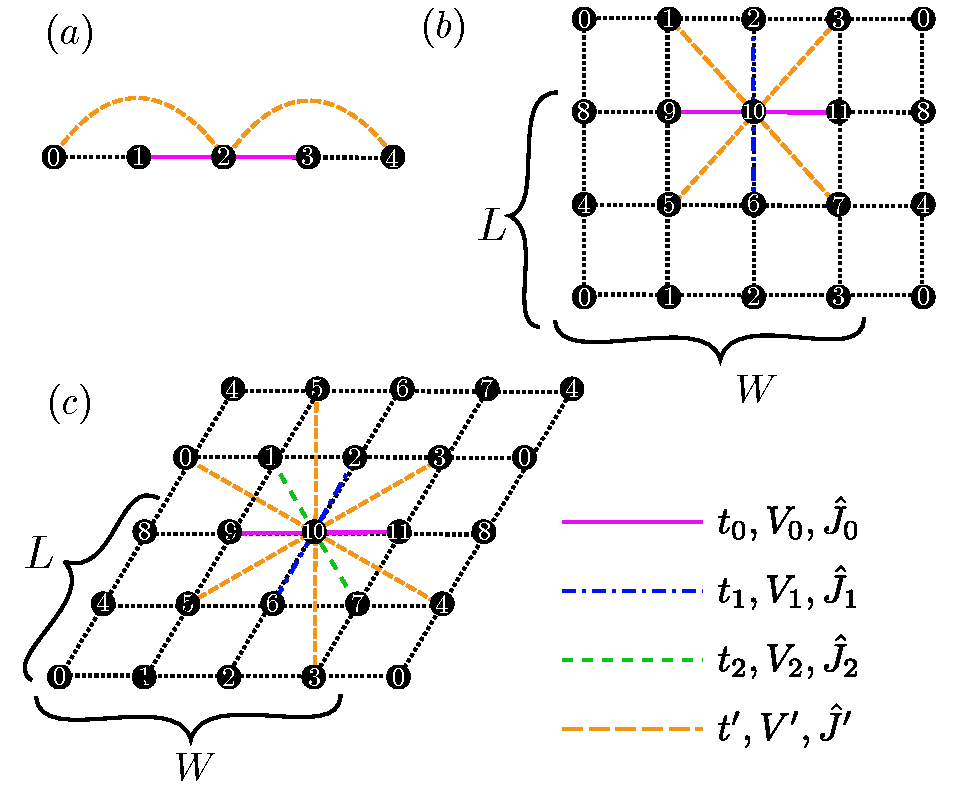
\includegraphics[width=10cm]{../figs/chap04_1_lattice.pdf}
    \caption{(a)1次元鎖、(b)2次元正方格子、(c)2次元三角格子の模式図. 
      ホッピング積分、オフサイトクーロン積分、スピン結合は、
      再近接サイト間(マゼンタの実線)ではそれぞれ$t,V,J$となり、
      次近接サイト間(緑の破線)ではそれぞれ$t',V',J'$となります。}
    \label{fig_chap04_1_lattice}
  \end{center}
\end{figure}

\begin{figure}[!htbp]
  \begin{center}
    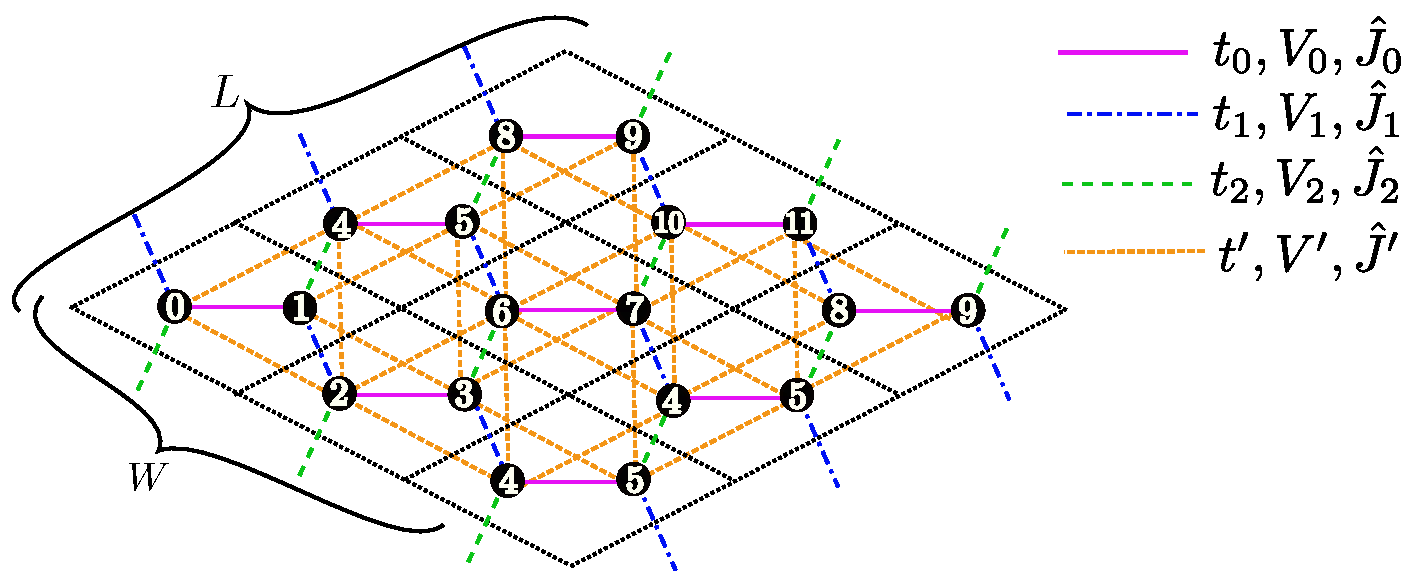
\includegraphics[width=15cm]{../figs/chap04_1_honeycomb.pdf}
    \caption{2次元異方的蜂の巣格子の模式図. 
      ホッピング積分、オフサイトクーロン積分、スピン結合は、
      ボンドの方向によって異なります。
      また、次近接のホッピング積分、オフサイトクーロン積分、スピン結合
      には対応していません。
    }
    \label{fig_chap04_1_honeycomb}
  \end{center}
\end{figure}

\begin{figure}[!htbp]
  \begin{center}
    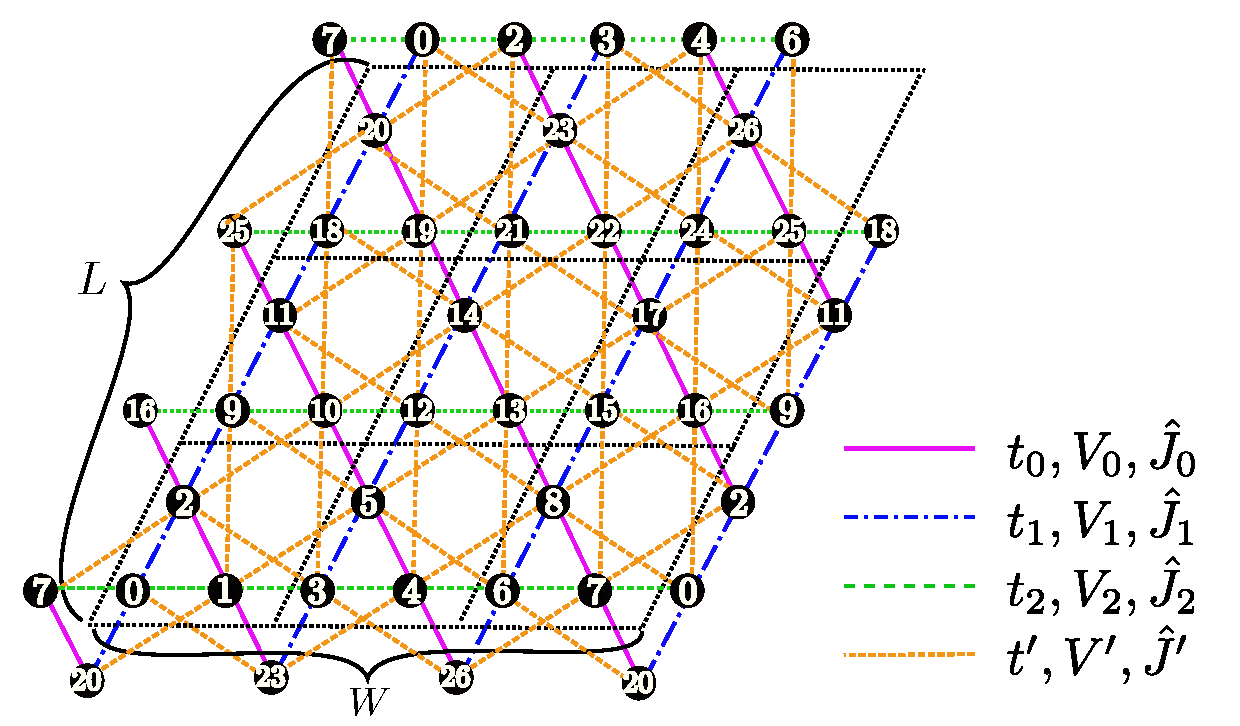
\includegraphics[width=15cm]{../figs/kagome.pdf}
    \caption{カゴメ格子の模式図. 
    }
    \label{fig_kagome}
  \end{center}
\end{figure}

\begin{figure}[!htbp]
  \begin{center}
    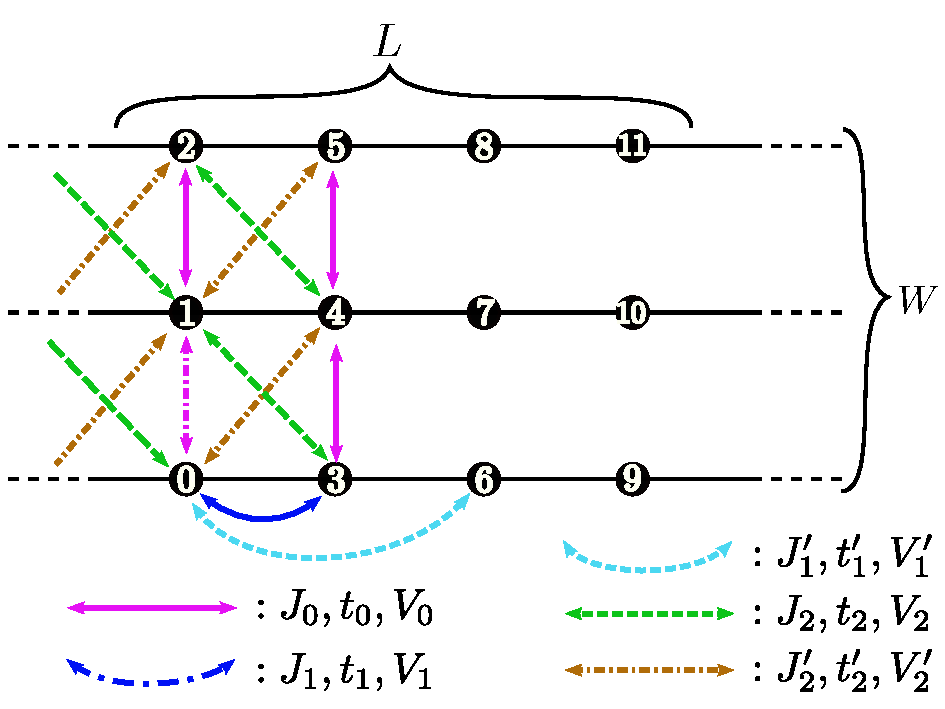
\includegraphics[width=10cm]{../figs/ladder.pdf}
    \caption{梯子格子の模式図. 
    }
    \label{fig_ladder}
  \end{center}
\end{figure}

\end{itemize}

\subsection{格子に関するパラメーター}

\subsubsection{1次元鎖[Fig. \ref{fig_chap04_1_lattice}(a)]}

\begin{itemize}

\item \verb|L|

{\bf 形式 :} 自然数

{\bf 説明 :} 鎖の長さを指定します. 

\end{itemize}

\subsubsection{梯子格子(Fig. \ref{fig_ladder})}

\begin{itemize}

\item \verb|L|

{\bf 形式 :} 自然数

{\bf 説明 :} 梯子の長さを指定します. 

\item \verb|W|

{\bf 形式 :} 自然数

{\bf 説明 :} 梯子の本数を指定します. 

\end{itemize}

\begin{figure}[!htbp]
  \begin{center}
    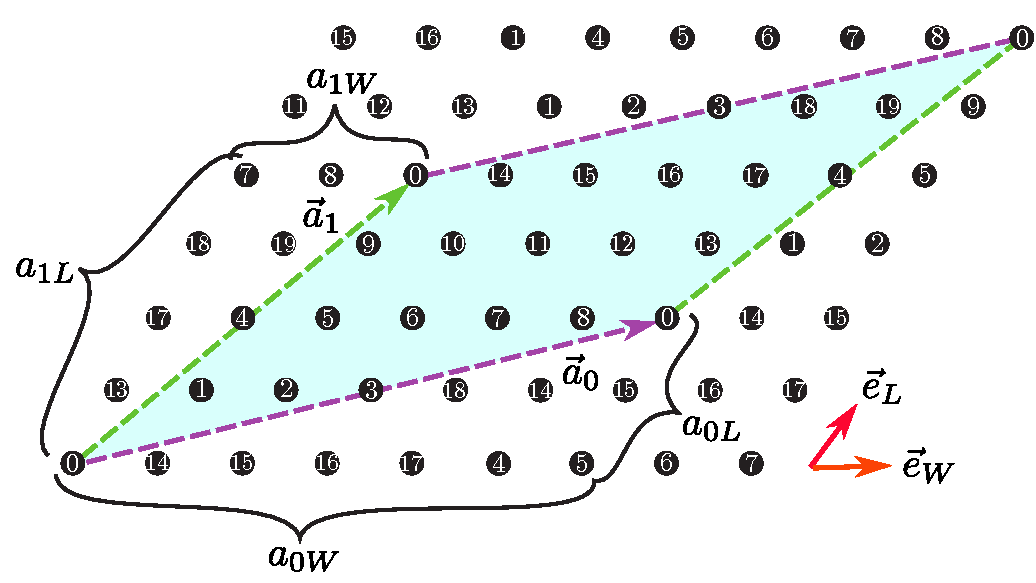
\includegraphics[width=15cm]{../figs/chap04_1_unitlattice.pdf}
    \caption{三角格子において、${\vec a}_0 = (6, 2), {\vec a}_1 = (2, 4)$とした場合のセル形状。
      ${\vec a}_0$(マゼンタ)および${\vec a}_1$(グリーン)
      で囲まれた部分(サイト数は20)が計算するセルとなる。
    }
    \label{fig_chap04_1_unitlattice}
  \end{center}
\end{figure}

\subsubsection{矩形格子[Fig. \ref{fig_chap04_1_lattice}(b)]、 
三角格子[Fig. \ref{fig_chap04_1_lattice}(c)]、
蜂の巣格子(Fig. \ref{fig_chap04_1_honeycomb})、
カゴメ格子(Fig. \ref{fig_kagome})}

これらの格子では、標準の単位胞(図中の黒の破線を参照)を用いて格子形状を指定する方法と、
それらとは別の方向に格子ベクトルを取る方法が選択できます。
ただし、\verb|model=SpinGCCMA|の時には前者のみが使えます。
また、両方を指定した場合には$\HPhi$を終了します。

\begin{itemize}

\item \verb|W|, \verb|L|

{\bf 形式 :} 自然数

{\bf 説明 :} 標準の単位胞の並び方を指定します。

\item \verb|a0W|, \verb|a0L|, \verb|a1W|, \verb|a1L|

{\bf 形式 :} 自然数

{\bf 説明 :} 格子を指定する2本のベクトル(${\vec a}_0, {\vec a}_1$)
を指定します (Fig. \ref{fig_chap04_1_unitlattice})。
これらのベクトルは標準の並進ベクトルを基底とした座標(Fractional coordinate)
で指定されます。

\end{itemize}

スタンダードモードで出力される\verb|lattice.gp|というファイルを使うと、
自分の意図した通りの格子のとり方になっているかどうかを確かめる事が出来ます。
このファイルは、次のようにして\verb|gnuplot|に読み込ませることが出来ます。
\begin{verbatim}
$ gnuplot lattice.gp
\end{verbatim}


\subsection{保存量に関するパラメーター}

\begin{itemize}
\item \verb|nelec|

{\bf 形式 :} 整数

{\bf 説明 :} 伝導電子数を指定します。
\verb|model = "Fermion HubbardGC"|, \verb|"Spin"|, \verb|"SpinGC"|
のときには指定しないでください。

\item \verb|2Sz|

{\bf 形式 :} 整数

{\bf 説明 :} 全スピンのz 成分の2倍を指定します。
\verb|model = "Fermion HubbardGC"|, \verb|SpinGC|
のときには指定しないでください。
\end{itemize}

\subsection{ハミルトニアンの各項の係数}

デフォルト値は特に記載されていないものについては0に設定してあります。
型が複素数のパラメータは「実部, 虚部」(間に``,'')の形式で指定し、
実数の場合には「実部」で指定が可能です。

\subsubsection{局所項}

\begin{itemize}

\item \verb|mu|

{\bf 形式 :} 実数

{\bf 説明 :} Hubbardおよび近藤格子模型での化学ポテンシャルを指定します。

\item \verb|U|

{\bf 形式 :} 実数

{\bf 説明 :} Hubbardおよび近藤格子模型でのオンサイトクーロン積分を指定します。

\item \verb|Jx|, \verb|Jy|, \verb|Jz|, \verb|Jxy|, 
  \verb|Jyx|, \verb|Jxz|, \verb|Jzx|, \verb|Jyz|, \verb|Jzy|

{\bf 形式 :} 実数

{\bf 説明 :} 近藤格子模型での、局在電子と遍歴電子のスピン結合を指定します。
また対角項について, \verb|Jx, Jy, Jz|を指定する代わりに、パラメータ\verb|J|を指定すると
\verb|Jx = Jy = Jz = J|が代入されます。
\verb|J|を指定した上で\verb|Jx|, \verb|Jy|, \verb|Jz|を指定した場合は$\HPhi$を終了します。

\item \verb|h|, \verb|Gamma|, \verb|D|

{\bf 形式 :} 実数

{\bf 説明 :} スピン模型での縦磁場、横磁場、異方性パラメータを指定します。
ただし異方性パラメータについては、\verb|model=SpinGCCMA|では使用できません。

\end{itemize}

下記の非局所項は、梯子格子の場合とそれ以外(1次元鎖、矩形格子、三角格子、蜂の巣格子、カゴメ格子)
の場合で指定の仕方が異なります。
また、各格子で指定可能なパラメーターをTable \ref{table_interactions}に表します。

\begin{table}[hbp]
  \begin{tabular}{|l||c|c|c|c|c|c|c|c|} \hline
    相互作用 & 1次元鎖 & 矩形格子 & 三角格子 & 蜂の巣格子 & カゴメ格子 & 梯子格子\\ 
    \hline \hline
     \verb|J|, \verb|t|, \verb|V|(省略形) & $\circ$	 & $\circ$ & $\circ$ & $\circ$ & $\circ$ & -\\ 
     \hline
    \verb|J'|, \verb|t'|, \verb|V'| & $\circ$	 & $\circ$	& $\circ$ 	& $\circ$ 	& $\circ$ & - \\ 
    \hline
    \verb|J0|, \verb|t0|, \verb|V0| & $\circ$  & $\circ$ 	& $\circ$ 	& $\circ$ 	& $\circ$ & $\circ$\\ 
    \hline
    \verb|J1|, \verb|t1|, \verb|V1| & -         	 & $\circ$ 	& $\circ$ 	& $\circ$ 	& $\circ$ & $\circ$\\ 
    \hline
    \verb|J2|, \verb|t2|, \verb|V2|  & -         	 & -    	& $\circ$ 	& $\circ$ 	& $\circ$ & $\circ$\\
    \hline
    \verb|J1'|, \verb|t1'|, \verb|V1'| & -		 &-	 	& -		& -		& -		& $\circ$\\
    \hline
    \verb|J2'| ,\verb|t2'|, \verb|V2'|  & -		 &-	 	& -		& -		& -		& $\circ$\\ 
    \hline
\end{tabular}
   \caption{各格子で定義可能な相互作用一覧。ただし、スピン結合については行列として与えることが可能。}
    \label{table_interactions}
\end{table}

\subsubsection{非局所項[梯子格子 (Fig. \ref{fig_ladder})]}

\begin{itemize}
\item \verb|t0|,  \verb|t1|,  \verb|t1'|,  \verb|t2|,  \verb|t2'|

{\bf 形式 :} 複素数

{\bf 説明 :} 梯子格子でのホッピング(Fig. \ref{fig_ladder}参照)を指定します。

\item \verb|V0|,  \verb|V1|,  \verb|V1'|,  \verb|V2|,  \verb|V2'|

{\bf 形式 :} 実数

{\bf 説明 :} 梯子格子でのオフサイトクーロン積分
(Fig. \ref{fig_ladder}参照)を指定します。

\item \verb|J0x|, \verb|J0y|, \verb|J0z|, \verb|J0xy|, 
  \verb|J0yx|, \verb|J0xz|, \verb|J0zx|, \verb|J0yz|, \verb|J0zy|
\item \verb|J1x|, \verb|J1y|, \verb|J1z|, \verb|J1xy|, 
  \verb|J1yx|, \verb|J1xz|, \verb|J1zx|, \verb|J1yz|, \verb|J1zy|
\item \verb|J1'x|, \verb|J1'y|, \verb|J1'z|, \verb|J1'xy|, 
  \verb|J1'yx|, \verb|J1'xz|, \verb|J1'zx|, \verb|J1'yz|, \verb|J1'zy|
\item \verb|J2x|, \verb|J2y|, \verb|J2z|, \verb|J2xy|, 
  \verb|J2yx|, \verb|J2xz|, \verb|J2zx|, \verb|J2yz|, \verb|J2zy|
\item \verb|J2'x|, \verb|J2'y|, \verb|J2'z|, \verb|J2'xy|, 
  \verb|J2'yx|, \verb|J2'xz|, \verb|J2'zx|, \verb|J2'yz|, \verb|J2'zy|

{\bf 形式 :} 実数

{\bf 説明 :} 梯子格子でのスピン相互作用
(Fig. \ref{fig_ladder}参照)を指定します。
また対角項について、例えば\verb|J0x, J0y, J0z|を指定する代わりに
パラメータ\verb|J0|を指定すると
\verb|J0x = J0y = J0z = J0|が代入されます。
\verb|J0|を指定した上で\verb|J0x, J0y, J0z|等も指定した場合は$\HPhi$を終了します。
\verb|J1|, \verb|J1'|, \verb|J2|, \verb|J2'|についても同様です。

\end{itemize}

\subsubsection{非局所項 [梯子格子以外(Figs. \ref{fig_chap04_1_lattice}, \ref{fig_chap04_1_honeycomb},
\ref{fig_kagome})]}

\begin{itemize}
\item \verb|t0|,  \verb|t1|, \verb|t2|

{\bf 形式 :} 複素数

{\bf 説明 :} Hubbardおよび近藤格子模型での、最近接サイト間の各方向のホッピングを指定します。
また、ホッピングのボンド方向依存性がない場合は\verb|t0|,  \verb|t1|, \verb|t2|を
別々に指定する代わりにパラメータ\verb|t|を指定すると、\verb|t0 = t1 = t2 = t|が代入されます。
\verb|t|と\verb|t0|等の両方が指定された場合には$\HPhi$を終了します。

\item \verb|V0|,  \verb|V1|, \verb|V2|

{\bf 形式 :} 実数

{\bf 説明 :} Hubbardおよび近藤格子模型での、最近接サイト間のCoulomb積分を指定します。
また、サイト間Coulomb積分のボンド方向依存性がない場合は\verb|V0|,  \verb|V1|, \verb|V2|を
別々に指定する代わりにパラメータ\verb|V|を指定すると、\verb|V0 = V1 = V2 = V|が代入されます。
\verb|V|と\verb|V0|等の両方が指定された場合には$\HPhi$を終了します。

\item \verb|J0x|, \verb|J0y|, \verb|J0z|, \verb|J0xy|, 
  \verb|J0yx|, \verb|J0xz|, \verb|J0zx|, \verb|J0yz|, \verb|J0zy|
\item \verb|J1x|, \verb|J1y|, \verb|J1z|, \verb|J1xy|, 
  \verb|J1yx|, \verb|J1xz|, \verb|J1zx|, \verb|J1yz|, \verb|J1zy|
\item \verb|J2x|, \verb|J2y|, \verb|J2z|, \verb|J2xy|, 
  \verb|J2yx|, \verb|J2xz|, \verb|J2zx|, \verb|J2yz|, \verb|J2zy|

{\bf 形式 :} 実数

{\bf 説明 :} スピン模型での、最近接サイト間のスピン相互作用を指定します。
また対角項について、例えば\verb|J0x, J0y, J0z|を指定する代わりに
パラメータ\verb|J0|を指定すると
\verb|J0x = J0y = J0z = J0|が代入されます。
\verb|J0|を指定した上で\verb|J0x, J0y, J0z|等も指定した場合は$\HPhi$を終了します。
\verb|J1|, \verb|J2|についても同様です。

スピン間相互作用のボンド方向依存性がない場合には、
\verb|Jx|, \verb|Jy|, \verb|Jz|, \verb|Jxy|, 
\verb|Jyx|, \verb|Jxz|, \verb|Jzx|, \verb|Jyz|, \verb|Jzy|
を指定すると、\verb|J0x = J1x = J2x = Jx|のようにすべてのボンド方向のスピン間相互作用に
同じ値を代入することが出来ます。
\verb|Jx|$\sim$\verb|Jzy|系列のどれかと\verb|J0x|$\sim$\verb|J2zy|系列のどれかを両方指定した
場合には$\HPhi$を終了します。
以下に最近接間スピン相互作用の指定方法の例を挙げます。

\begin{itemize}

\item ボンド方向依存性、スピン方向依存性、相互作用の非対角成分($J_{x y}$等)がない場合

\verb|J|を指定

\item ボンド方向依存性、相互作用の非対角成分がなく、スピン方向依存性がある場合

\verb|Jx, Jy, Jz|のうち\verb|0|でないものを指定

\item ボンド方向依存性がなく、スピン方向依存性、相互作用の非対角成分がある場合

\verb|Jx, Jy, Jz, Jxy, Jyz, Jxz, Jyx, Jzy, Jzx|のうち\verb|0|でないものを指定

\item スピン方向依存性、相互作用の非対角成分がなく、ボンド方向依存性がある場合

\verb|J0, J1, J2|のうち\verb|0|でないものを指定

\item スピン方向依存性がなく、ボンド方向依存性、相互作用の非対角成分がある場合

\verb|J0x, J0y, J0z, J1x, J1y, J1z, J2x, J2y, J2z|のうち\verb|0|でないものを指定

\item ボンド方向依存性、スピン方向依存性、相互作用の非対角成分がある場合

\verb|J0x|$\sim$\verb|J2zy|のすべてのうち\verb|0|でないものを指定

\end{itemize}
\item \verb|t'|

{\bf 形式 :} 複素数

{\bf 説明 :} Hubbardおよび近藤格子模型での、次近接サイト間の各方向のホッピングを指定します。

\item \verb|V'|

{\bf 形式 :} 実数

{\bf 説明 :} Hubbardおよび近藤格子模型での、次近接サイト間のCoulomb積分を指定します。

\item \verb|J'x|, \verb|J'y|, \verb|J'z|, \verb|J'xy|, 
  \verb|J'yx|, \verb|J'xz|, \verb|J'zx|, \verb|J'yz|, \verb|J'zy|

{\bf 形式 :} 実数

{\bf 説明 :} スピン模型での、次近接サイト間のスピン相互作用を指定します。
ただし、蜂の巣格子またはカゴメ格子で\verb|model=SpinGCCMA|の場合には
まだ対応していません。
また対角項について、\verb|J'x, J'y, J'z|を指定する代わりに
パラメータ\verb|J'|を指定すると
\verb|J'x = J'y = J'z = J'|が代入されます。
\verb|J'|を指定した上で\verb|J'x, J'y, J'z|も指定した場合は$\HPhi$を終了します。

\item \verb|phase0|, \verb|phase1|

  {\bf 形式 :} 実数 (デフォルトでは\verb|0.0|)
  
  {\bf 説明 :} 計算するセルの境界をまたいだホッピング項に付く因子の位相を指定することが出来ます
  (単位: 度)。
  $\vec{a}_0$方向、$\vec{a}_1$方向それぞれ別の位相因子を用いることが出来ます。
  1次元系では\verb|phase0|のみ使用できます。
  例えば、$i$サイトから$j$サイトへのホッピングで、
  正の方向に境界をまたいだ場合には次のようになります。
  \begin{align}
    \exp(i \times {\rm phase0}\times\pi/180) \times t {\hat c}_{j \sigma}^\dagger {\hat c}_{i \sigma}
    + \exp(-i \times {\rm phase0}\times\pi/180) \times t^* {\hat c}_{i \sigma}^\dagger {\hat c}_{j \sigma}
  \end{align}

\end{itemize}

\subsection{計算条件のパラメーター}

\begin{itemize}
\item \verb|2S|

{\bf 形式 :} 正の整数(デフォルト値は\verb|1|)

{\bf 説明 :} スピン模型での局在スピンの大きさ$S$の2倍を指定します。
(例/ $1/2$スピンならば\verb|1|)

\item \verb|Restart|

  {\bf 形式 :} 文字列(\verb|"None"|, \verb|"Restart_out"|, \verb|"Restart_in"|,  
  \verb|"Restart"|のいずれか。デフォルトは\verb|"None"|)

  {\bf 説明 :} 再計算に関する設定を行う。
  \verb|"None"|では再計算に関連するファイル出力をしない。
  \verb|"Restart_out"|では一から計算を始めて、
  反復が終了した時点で再計算用のデータをファイル出力する。
  \verb|"Restart_in"|では再計算用のデータをファイルから受け取り途中から計算を始める。
  \verb|"Restart"|では再計算用のデータをファイルから受け取り途中から計算を始め、
  反復が終了した時点で再計算用のデータをファイル出力する。

\item \verb|Lanczos_max|

{\bf 形式 :} 整数(デフォルト値は\verb|2000|)

{\bf 説明 :} ランチョスステップの上限、LOBCGステップの上限、
TPQステップ数、時間発展ステップ数、BiCGステップの上限を指定します。

\item \verb|initial_iv|

{\bf 形式 :} 整数(デフォルト値は\verb|-1|)

{\bf 説明 :}  {初期条件のベクトルを与えます。}
\begin{itemize}
\item{ランチョス法}
\begin{itemize}
\item{カノニカル集団かつ \verb|initial_iv| $\geq 0$の場合}

ノンゼロの成分が指定されます。

\item{ \verb|initial_iv| $< 0$の場合}

乱数のシードが指定され、全ての成分に対して係数がランダムに与えられます。なお、グランドカノニカルの場合は初期状態として多くの状態を持つよう、こちらの様式が適用されます。
\end{itemize}

\item{TPQ法}

乱数のシードが指定され、全ての成分に対して係数がランダムに与えられます。
\end{itemize}
初期ベクトル設定の詳細については、\ref{Ch:algorithm}を参照ください。

%\item \verb|nvec|

%{\bf 形式 :} 整数(デフォルト値は\verb|1|)

%{\bf 説明 :} ランチョス法の段階で下からいくつの固有値を求めるかを指定します。

\item \verb|exct|

{\bf 形式 :} 整数(デフォルト値は\verb|1|)

{\bf 説明 :}
\verb|method="Lancoz"|ではエネルギーの低いものから数えて、
何番目の固有状態を計算するかを指定します。
\verb|method="CG"|の時には求める固有状態の本数を指定します。

\item \verb|LanczosEps|

{\bf 形式 :} 整数(デフォルト値は\verb|14|)

{\bf 説明 :} ランチョスの収束判定条件を指定します。
ひとつ前のステップの固有値との相対誤差が,
$10^{-{\tt LanczosEps}}$以下になったら収束したと判断します。
\verb|method="CG"|の時には残差ベクトルの2-ノルムが
$10^{-{\tt LanczosEps}/2}$以下になったら収束したと判断します。

\item \verb|LancczosTarget|

{\bf 形式 :} 整数(デフォルト値は\verb|2|)

{\bf 説明 :} エネルギーの低いものから数えて、
何番目の固有値でランチョスの収束判定を行うかを指定します。

\item \verb|LargeValue|

{\bf 形式 :} 実数(デフォルト値は下記参照)

{\bf 説明 :} (TPQ法のみで使用)$l-\hat{H}/N_{s}$の$l$。
ハミルトニアンの各項の係数の絶対値の総和をサイト数で割ったものがデフォルト値になります。

%\begin{itemize}

%\item Hubbard模型[式(\ref{fml4_1_hubbard})]

%カノニカル集団
%\begin{align}
%l = |\mu| \frac{N_{\rm elec}}{N_{\rm site}}
%+ 2 z |t| + 2 z' |t'| + |U| + 2 z |V| + 2 z' |V'| 
%\end{align}
%グランドカノニカル集団
%\begin{align}
%l = 2|\mu|
%+ 2 z |t| + 2 z' |t'| + |U| + 2 z |V| + 2 z' |V'|
%\end{align}

%\item スピン模型[式(\ref{fml4_1_spin})]

%カノニカル集団
%\begin{align}
%l = \frac{|S_z^{\rm tot}|}{N_{\rm site}}|h| + S |\Gamma| + S^2 |D|
%+\frac{z}{2} S^2 (|J_x|+|J_y|+|J_z|) +\frac{z'}{2} S^2 (|J'_x|+|J'_y|+|J'_z|)
%\end{align}
%グランドカノニカル集団
%\begin{align}
%l = S |h| + S |\Gamma| + S^2 |D|
%+\frac{z}{2} S^2 (|J_x|+|J_y|+|J_z|) + \frac{z'}{2} S^2 (|J'_x|+|J'_y|+|J'_z|) 
%\end{align}
%
%\item 近藤格子模型[式(\ref{fml4_1_kondo})]
%
%カノニカル集団
%\begin{align}
%l = |\mu| \frac{N_{\rm elec}}{N_{\rm site}} + 2 z |t| + \frac{S}{2} |J| 
%\end{align}
%グランドカノニカル集団
%\begin{align}
%l = 2|\mu| + 2 z |t| + \frac{S}{2} |J| 
%\end{align}
%
%\end{itemize}

\item \verb|NumAve|

{\bf 形式 :} 整数(デフォルト値は\verb|5|)

{\bf 説明 :} (TPQ法のみで使用)独立なrunを何回行うかを指定します。

\item \verb|ExpecInterval|

{\bf 形式 :} 整数(デフォルト値は\verb|20|)

{\bf 説明 :} (TPQ法のみで使用)相関関数の計算を何回のTPQステップおきに行うかの指定。
頻度を上げると計算コストが増大するので注意してください。

\item \verb|OutputMode|

{\bf 形式 :} \verb|"none"|, \verb|"correlation"|, \verb|"full"|のいずれか(デフォルトは\verb|correlation|)

{\bf 説明 :} 計算を行う相関関数を指定します。
\verb|"none"|の場合は相関関数を計算しません。
\verb|"correlation"|を指定した場合には、付属のユーティリティ
\verb|fourier|でサポートするものに対応した相関関数を計算します。
詳しくは\verb|doc/fourier/|内のマニュアルを参照してください。
\verb|"full"|を指定した場合には、
1体部分はすべての$i, j, \sigma, \sigma'$について
$\langle c_{i \sigma}^{\dagger}c_{j \sigma'} \rangle$を、
2体部分はすべての$i_1, i_2, i_3, i_4, \sigma_1, \sigma_2, \sigma_3, \sigma_4$について
$\langle c_{i_1 \sigma_1}^{\dagger}c_{i_2 \sigma_2} c_{i_3 \sigma_3}^{\dagger}c_{i_4 \sigma_4} \rangle$
を計算します。
スピン系の演算子はBogoliubov表現により生成消滅演算子で表されています。
詳しくは\ref{sec_bogoliubov_rep}をご覧ください。

\item \verb|InitialVecType|

  {\bf 形式 :} 文字 (\verb|"C"|, \verb|"R"|のいずれか。
  デフォルトは\verb|"C"|)

  {\bf 説明 :} 固有ベクトルの初期値の型を指定する。
  \verb|C|では複素数型、\verb|R|では実数型とする。

\item \verb|EigenVecIO|
  
  {\bf 形式 :} 文字列(\verb|"None"|, \verb|"Out"|, \verb|"In"|のいずれか。
  デフォルトは\verb|"None"|)

  {\bf 説明 :} 固有ベクトルの入出力を指定する。
  \verb|"None"|では固有ベクトルの入出力を行わない。
  \verb|"Out"|では求めた固有ベクトルをファイルに出力する。
  \verb|"In"|では固有ベクトルをファイルから取り出し、
  その後の計算(動的グリーン関数など)を行う。

\end{itemize}

\subsection{動的グリーン関数の計算に関するパラメーター}

\begin{itemize}
\item \verb|CalcSpec|
  
  {\bf 形式 :} 文字列(\verb|"None"|, \verb|"Normal"|, \verb|"NoIteration"|,  
  \verb|"Restart_out"|, \verb|"Restart_in"|, \verb|"Restart"|。デフォルトは\verb|"None"|)

  {\bf 説明 :} 動的グリーン関数の計算に関する設定を行う。
  \verb|"None"|では動的グリーン関数を計算しない。
  \verb|"Normal"|では一から動的グリーン関数の計算を始める。
  \verb|"NoIteration"|では、前回の反復回数と同じところまで反復させる。
  このとき、ハミルトニアン-ベクトル積演算は行われないため、
  計算コストは非常に軽いが、十分な精度が出せない場合がある。
  \verb|"Restart_out"|では一から計算を始めて、
  反復が終了した時点で再計算用のデータをファイル出力する。
  \verb|"Restart_in"|では再計算用のデータをファイルから受け取り途中から計算を始める。
  \verb|"Restart"|では再計算用のデータをファイルから受け取り途中から計算を始め、
  反復が終了した時点で再計算用のデータをファイル出力する。
  スペクトル計算において使用される手法はパラメーター\verb|method|で指定されます。
  (\verb|method="CG"|とした場合には
  付属している$K\omega$ライブラリ\cite{komega}が呼び出され、
  シードスイッチ付きシフト双共役勾配法
  \cite{Frommer2003,doi:10.1143/JPSJ.77.114713}が使われます。

\item \verb|SpectrumType|
  
  {\bf 形式 :} 文字列(\verb|"SzSz"|, \verb|"S+S-"|, \verb|"Density"|,  
  \verb|"up"|, \verb|"down"|のいずれか。デフォルトは\verb|"SzSz"|)

  {\bf 説明 :} 計算する動的グリーン関数の種類を指定する。
  \verb|"SzSz"|では$\langle {\hat S}_{z q} {\hat S}_{z q}\rangle$、
  \verb|"S+S-"|では$\langle {\hat S}^{+}_{q} {\hat S}^{-}_{q}\rangle$、
  \verb|"Density"|では$\langle {\hat n}_{q} {\hat n}_{q}\rangle$、
  \verb|"up"|では$\langle {\hat c}^{\dagger}_{q \uparrow} {\hat c}_{q \uparrow}\rangle$、
  \verb|"down"|では$\langle {\hat c}^{\dagger}_{q \downarrow} {\hat c}_{q \downarrow}\rangle$
  となる。

\item \verb|SpectrumQW|, \verb|SpectrumQL|
  
  {\bf 形式 :} 実数(デフォルトはともに\verb|0.0|)

  {\bf 説明 :} 計算する動的グリーン関数の波数を
  Fractional coordinateで指定する。
  逆格子ベクトルはFigs.
  \ref{fig_chap04_1_lattice}, \ref{fig_chap04_1_honeycomb},
  \ref{fig_ladder}, \ref{fig_kagome}
  に表されている格子ベクトルと対応するものとなる。

\item \verb|OmegaMin|

  {\bf 形式 :} 実数(デフォルトは\verb|-LargeValue|$\times$サイト数)
  
  {\bf 説明 :} 計算する動的グリーン関数の振動数の実部の下限。
    
\item \verb|OmegaMax|

  {\bf 形式 :} 実数(デフォルトは\verb|LargeValue|$\times$サイト数)
  
  {\bf 説明 :} 計算する動的グリーン関数の振動数の実部の上限。

\item \verb|OmegaIm|

  {\bf 形式 :} 実数(デフォルトは\verb|0.01*LargeValue|)
  
  {\bf 説明 :} 計算する動的グリーン関数の振動数の虚部。

\item \verb|NOmega|
  
  {\bf 形式 :} 正の整数(デフォルトは\verb|200|)
    
  {\bf 説明 :} 計算する動的グリーン関数の振動数のグリッド数。

\end{itemize}

\subsection{実時間発展計算に関するパラメーター}

\begin{itemize}

\item \verb|dt|
  
  {\bf 形式 :} 正の実数(デフォルトは\verb|0.1|)
  
  {\bf 説明 :} 時間ステップ幅。

\item \verb|PumpType|
  
  {\bf 形式 :} 文字列(\verb|"Quench"|, \verb|"Pulse Laser"|, \verb|"AC Laser"|,  
  \verb|"DC Laser"|のいずれか。デフォルトは\verb|"Quench"|)

  {\bf 説明 :} 時間依存ハミルトニアンの種類を指定する。
  \verb|"Quench"|では2体演算子
  $U_{\rm quench} \sum_i n_{i \uparrow} n_{i \downarrow}$が加えられる。
  \verb|"Pulse Laser"|, \verb|"AC Laser"|, \verb|"DC Laser"|では、
  ホッピング項に
  $-\sum_{i j \sigma} t_{i j} \exp[-i{\bf A}(t) \cdot ({\bf R}_i-{\bf R}_j)/(2\pi)] c_{i \sigma} c_{j \sigma}$
  のように位相因子が付く。
  ここで${\bf A}(t)$はベクトルポテンシャルであり、
  \verb|"Pulse Laser"|では
  ${\bf A}(t) = {\bf A}_0 \exp[-(t-t_0)^2/(2 t_{\rm dump}^2)] \cos[\omega (t-t_0)]$、
  \verb|"AC Laser"|では
  ${\bf A}(t) = {\bf A}_0 \sin[\omega (t-t_0)]$、
  \verb|"DC Laser"|では
  ${\bf A}(t) = {\bf A}_0 t$となる。

  また、各時刻でのベクトルポテンシャルと電場を図示するためのファイル
  \verb|potential.dat|が出力される。
  
\item \verb|Uquench|
  
  {\bf 形式 :} 実数(デフォルトは\verb|0.0|)
  
  {\bf 説明 :} $U_{\rm quench}$

\item \verb|freq|
  
  {\bf 形式 :} 実数(デフォルトは\verb|0.1|)
  
  {\bf 説明 :} $\omega$

\item \verb|tshift|
  
  {\bf 形式 :} 実数(デフォルトは\verb|0.0|)
  
  {\bf 説明 :} $t_0$

\item \verb|tdump|
  
  {\bf 形式 :} 実数(デフォルトは\verb|0.1|)
  
  {\bf 説明 :} $t_{\rm dump}$

\item \verb|VecPotW|, \verb|VecPotL|
  
  {\bf 形式 :} 実数(デフォルトはともに\verb|0.0|)

  {\bf 説明 :} 時刻$t=t_0$でのベクトルポテンシャル${\bf A}_0$を
  逆格子のFractional coordinateで指定する。
  逆格子ベクトルはFigs.
  \ref{fig_chap04_1_lattice}, \ref{fig_chap04_1_honeycomb},
  \ref{fig_ladder}, \ref{fig_kagome}
  に表されている格子ベクトルと対応するものとなる。

\end{itemize}

\newpage
\section{エキスパートモード用入力ファイル}
\label{Ch:HowToExpert}

$\HPhi$のエキスパートモードで使用する入力ファイル(*def)に関して説明します。
入力ファイルの種別は以下の4つで分類されます。
\begin{description}
\item[(1)~List:]
~\\{キーワード指定なし}:
使用するinput fileの名前のリストを書きます。なお、ファイル名は任意に指定することができます。
\item[(2)~Basic parameters:]
~\\{\bf CalcMod}: 計算モードを指定するパラメーターを設定します。
~\\{\bf ModPara}: 計算時に必要な基本的なパラメーター(サイトの数、電子数、Lanczosステップを何回やるかなど)を設定します。
~\\{\bf LocSpin}: 局在スピンの位置を設定します(近藤模型でのみ利用)。
\item[(3)~Hamiltonian:] 
$\HPhi$のHamiltonianを電子系の表式により指定します。
~\\具体的には以下のファイルで指定されます。
~\\{\bf Trans}: $c_{i\sigma_1}^{\dag}c_{j\sigma_2}$で表される一体項を指定します。
~\\{\bf InterAll}: $c_ {i \sigma_1}^{\dag}c_{j\sigma_2}c_{k \sigma_3}^{\dag}c_{l \sigma_4}$で表される一般二体相互作用を指定します。\\
~\\なお、使用頻度の高い相互作用に関しては下記のキーワードで指定することも可能です。
~\\{\bf CoulombIntra}: $n_ {i \uparrow}n_{i \downarrow}$で表される相互作用を指定します($n_{i \sigma}=c_{i\sigma}^{\dag}c_{i\sigma}$)。
~\\{\bf CoulombInter}: $n_ {i}n_{j}$で表される相互作用を指定します($n_i=n_{i\uparrow}+n_{i\downarrow}$)。
~\\{\bf Hund}: $n_{i\uparrow}n_{j\uparrow}+n_{i\downarrow}n_{j\downarrow}$で表される相互作用を指定します。
~\\{\bf PairHop}:  $c_ {i \uparrow}^{\dag}c_{j\uparrow}c_{i \downarrow}^{\dag}c_{j  \downarrow}$で表される相互作用を指定します。
~\\{\bf Exchange}: $S_i^+ S_j^-$で表される相互作用を指定します。
~\\{\bf Ising}: $S_i^z S_j^z$で表される相互作用を指定します。
~\\{\bf PairLift}: $c_ {i \uparrow}^{\dag}c_{i\downarrow}c_{j \uparrow}^{\dag}c_{j \downarrow}$で表される相互作用を指定します。
\item[(4)~Output:]
~\\{\bf OneBodyG }:出力する一体Green関数を指定します。
 $\langle c^{\dagger}_{i\sigma_1}c_{j\sigma_2}\rangle$が出力されます。

 {\bf TwoBodyG }:出力する二体Green関数を指定します。
 $\langle c^{\dagger}_{i\sigma_1}c_{j\sigma_2}c^{\dagger}_{k \sigma_3}c_{l\sigma_4}\rangle$
が出力されます。
\end{description}
%%%%%%%%%%%%%%%%%%%%%%
\newpage
~\subsection{入力ファイル指定用ファイル}
\label{Subsec:InputFileList}
計算で使用する入力ファイル一式を指定します。ファイル形式に関しては、以下のようなフォーマットをしています。\\
\begin{minipage}{10cm}
\begin{screen}
\begin{verbatim}
CalcMod  calcmod.def
ModPara  modpara.def
LocSpin  zlocspn.def
Trans    ztransfer.def
InterAll zinterall.def
OneBodyG zcisajs.def
TwoBodyG	zcisajscktaltdc.def
\end{verbatim}
\end{screen}
\end{minipage}
\\
\subsubsection{ファイル形式}
[string01]~[string02]
\subsubsection{パラメータ}
 \begin{itemize}
   \item  $[$string01$]$
   
   {\bf 形式 :} string型 (固定)
   
   {\bf 説明 :} キーワードを指定します。
   
   \item  $[$string02$]$
   
    {\bf 形式 :} string型 

   {\bf 説明 :} キーワードにひも付けられるファイル名を指定します(任意)。
 \end{itemize}
\subsubsection{使用ルール}
本ファイルを使用するにあたってのルールは以下の通りです。
\begin{itemize}
\item キーワードを記載後、半角空白を開けた後にファイル名を書きます。ファイル名は自由に設定できます。
\item ファイル読込用キーワードはTable\ref{Table:Defs}により指定します。
\item 必ず指定しなければいけないパラメーターはCalcMod, ModPara, LocSpinです。
\item 各キーワードは順不同に記述できます。
\item 指定したキーワード、ファイルが存在しない場合はエラー終了します。
\item $\#$で始まる行は読み飛ばされます。
\end{itemize}

 \begin{table*}[h!]
\begin{center}
  \begin{tabular}{ll|} \hline
           Keywords     & 指定ファイルの概要       \\   \hline\hline
           CalcMod      &   計算モードに関する指定をします。  \\  \hline  
           ModPara       &  計算で用いるパラメータの指定をします。  \\ \hline   
           LocSpin         &  各サイトに対して遍歴電子もしくは局在スピンの指定をします。        \\ 
           Trans       &   一般的一体相互作用に関する設定をします。  \\
           InterAll  &   一般的二体相互作用に関する設定をします。 \\  
           CoulombIntra  &   内部クーロン相互作用に関する設定をします。 \\  
           CoulombInter  &   サイト間クーロン相互作用に関する設定をします。\\  
           Hund  &   フント結合に関する設定をします。 \\  
           PairHop  &  ペアホッピングに関する設定をします。 \\  
           Exchange  &  交換相互作用に関する設定をします。 \\  
           Ising  &  イジング相互作用に関する設定をします。 \\  
           PairLift  &   ペアリフト相互作用に関する設定をします。 \\  
           OneBodyG         &   出力する一体グリーン関数$\langle c_{i\sigma}^{\dagger}c_{j\sigma}\rangle$ に関する設定をします。\\   
           TwoBodyG &   出力するニ体グリーン関数 $\langle c_{i\sigma}^{\dagger}c_{j\sigma}c_{k\tau}^{\dagger}c_{l\tau}\rangle$に関する設定をします。 \\   
           {SingleExcitation} &   一体励起状態の生成演算子に関する指定をします。\\ 
           {PairExcitation} &   ニ体励起状態の生成演算子に関する指定をします。\\   
           {SpectrumVec} &   スペクトル関数を計算するためのリスタート用の入力ベクトルを指定します。\\   
           \hline
  \end{tabular}
\end{center}
\caption{List of the definition files.}
\label{Table:Defs}
\end{table*}%

\newpage
%----------------------------------
\subsection{CalcModファイル}
\label{Subsec:calcmod}
計算手法、計算モデル、出力モードを指定します。以下のようなフォーマットをしています。\\
\begin{minipage}{10cm}
\begin{screen}
\begin{verbatim}
CalcType   0
CalcModel   2
CalcEigenVec 0
\end{verbatim}
\end{screen}
\end{minipage}
\\
%----------------------------------
\subsubsection{ファイル形式}
[string01]~[int01]
\subsubsection{パラメータ}
 \begin{itemize}
   \item  $[$string01$]$
   
   {\bf 形式 :} string型 (固定)
   
   {\bf 説明 :} キーワードを指定します。
   
   \item  $[$int01$]$
   
    {\bf 形式 :} int型 

   {\bf 説明 :} キーワードにひも付けられるパラメータを指定します。\\

   
  \end{itemize}

\subsubsection{使用ルール}
本ファイルを使用するにあたってのルールは以下の通りです。
\begin{itemize}
\item キーワードを記載後、半角空白を開けた後に整数値を書きます。
\item 各キーワードは順不同に記述できます。
\item 指定したキーワード、ファイルが存在しない場合はエラー終了します。
\item キーワードCalcType, CalcModelは省略できません。 省略した場合はエラー終了します。
\item $\#$で始まる行は読み飛ばされます。
\end{itemize}
~\subsubsection{キーワード}
次に各キーワードで指定されるパラメータに関して説明します。
\begin{itemize}
\item  \verb|CalcType|

{\bf 形式 :} int型 

{\bf 説明 :} 計算手法の指定を行います。\\
0: Lanczos法\\
1: TPQを利用した有限温度解析\\
2: 全対角化\\
3: LOBCG法\\
を選択することができます。

\item  \verb|CalcModel|

{\bf 形式 :} int型 

{\bf 説明 :} 計算モデルの指定を行います。\\
0: fermion Hubbard模型(カノニカル:粒子数・$S_z$保存、{粒子数・$S_z$非保存})\\
1: スピン模型(カノニカル:$S_z$保存)\\
2: 近藤模型(カノニカル:粒子数・$S_z$保存)\\
3: fermion Hubbard模型(グランドカノニカル:粒子数・$S_z$非保存)\\
4: スピン模型(グランドカノニカル:$S_z$非保存)\\
5: 近藤模型(グランドカノニカル:粒子数・$S_z$非保存)\\
を選択することが出来ます。
{ferimon Hubbard模型で粒子数保存・$S_z$非保存を選択する場合は、粒子数のみを指定することで計算が可能となります。}

\item  \verb|CalcEigenVec|

{\bf 形式 :} int型 (デフォルト値 0)

{\bf 説明 :} 固有ベクトルを計算する際の手法の指定を行います。\\
0: Lanczos法+CG法 (Lanczos法での収束が十分でない場合にCG法での固有ベクトル計算が行われます)\\
1: Lanczos法\\
で選択することが出来ます。

\item  \verb|InitialVecType|

{\bf 形式 :} int型 (デフォルト値 0)

{\bf 説明 :} 固有ベクトルの初期値の型の指定を行います。\\
0: 複素数\\
1: 実数\\
から選択することが出来ます。

\item  \verb|OutputEigenVec|

{\bf 形式 :} {int型 (デフォルト値 0)}

{\bf 説明 :} {固有ベクトルの出力の指定を行います。\\
0: 出力なし\\
1: 出力あり\\
から選択することが出来ます。}

\item  \verb|InputEigenVec|

{\bf 形式 :} {int型 (デフォルト値 0)}

{\bf 説明 :} {固有ベクトルの入力の指定を行います。\\
0: 入力なし\\
1: 入力あり\\
から選択することが出来ます。}

\item  \verb|ReStart|

{\bf 形式 :} {int型 (デフォルト値 0)}

{\bf 説明 :} {
{
再計算用のモードを指定します。\\
0: 再計算なし\\
1: リスタートベクトル入力なし、出力あり\\
2: リスタートベクトル入力あり、出力あり\\
3: リスタートベクトル入力あり、出力なし\\
から選択することが出来ます。
}
}

\item  \verb|CalcSpec|

{\bf 形式 :} {int型 (デフォルト値 0)}

{\bf 説明 :} {
{
動的グリーン関数の計算モードを指定します。\\
0: 動的グリーン関数の計算なし\\
1: 入力ベクトル・励起状態生成ファイルを読み込み計算\\
2: 三重対角行列の成分を読み込み再計算\\
3: 三重対角行列の成分と再計算用ベクトルを出力\\
4: 三重対角行列の成分と再計算用ベクトルを読み込み再計算\\
5: 三重対角行列の成分と再計算用ベクトルを読み込み再計算・再出力\\
から選択することが出来ます。}
}

\item  \verb|OutputHam|

{\bf 形式 :} {int型 (デフォルト値 0)}

{\bf 説明 :} {
{
(FullDiag) ハミルトニアンの出力モードを指定します。\\
0: 出力なし\\
1: 出力あり\\
から選択することが出来ます。}
}

\item  \verb|InputHam|

{\bf 形式 :} {int型 (デフォルト値 0)}

{\bf 説明 :} {
{
(FullDiag) ハミルトニアンの入力モードを指定します。\\
0: 入力なし\\
1: 入力あり\\
から選択することが出来ます。}
}

\item  \verb|Scalapack|

{\bf 形式 :} int型 (デフォルト値 0)

{\bf 説明 :} (FullDiag) 全対角化計算でのScaLAPACKライブラリの使用有無を指定します。\\
0: ScaLAPACKを使用しない。\\
1: ScaLAPACKを使用する。\\
で選択することが出来ます。

\item  \verb|NGPU|

{\bf 形式 :} int型 (デフォルト値 2)

{\bf 説明 :} (FullDiag) 全対角化計算でのMAGMAライブラリを使用する場合のGPU数を指定します。
なお、$\HPhi$ではマルチノードでのGPU計算には対応していません。

\end{itemize}

\newpage
\subsection{{ModParaファイル}}
\label{Subsec:modpara}
計算で使用するパラメータを指定します。以下のようなフォーマットをしています。\\
\begin{minipage}{10cm}
\begin{screen}
\begin{verbatim}
--------------------
Model_Parameters   0
--------------------
HPhi_Cal_Parameters
--------------------
CDataFileHead  zvo
CParaFileHead  zqp
--------------------
Nsite          16   
Ncond          16    
2Sz            0    
Lanczos_max    1000 
initial_iv     12   
exct           1    
LanczosEps     14   
LanczosTarget  2    
LargeValue     12   
NumAve         5    
ExpecInterval  20   
\end{verbatim}
\end{screen}
\end{minipage}

\subsubsection{ファイル形式}
以下のように行数に応じ異なる形式をとります。
 \begin{itemize}
   \item  1 - 5行:  ヘッダ(何が書かれても問題ありません)。
   \item  6行:  [string01]~[string02]
   \item  7 - 8行: ヘッダ(何が書かれても問題ありません)
   \item  9行以降: [string01]~[int01]
  \end{itemize}
各項目の対応関係は以下の通りです。
\begin{itemize}
   \item  $[$string01$]$
   
   {\bf 形式 :} string型 (固定)

  {\bf 説明 :} キーワードの指定を行います。
   
   \item  $[$string02$]$
   
   {\bf 形式 :} string型 (空白不可)

  {\bf 説明 :} アウトプットファイルのヘッダを指定します。

   \item  $[$int01$]$
   
   {\bf 形式 :} int型 (空白不可)

  {\bf 説明 :} キーワードでひも付けられるパラメータを指定します。

  \end{itemize}

\subsubsection{使用ルール}
本ファイルを使用するにあたってのルールは以下の通りです。
\begin{itemize}
\item 9行目以降ではキーワードを記載後、半角空白を開けた後に整数値を書きます。
\item 行数固定で読み込みを行う為、パラメータの省略はできません。
\end{itemize}

~\subsubsection{キーワード}
以下、共通パラメータと各手法毎に必要なパラメータを記載します。

~\subsubsection{共通パラメータ}

 \begin{itemize}
  \item  \verb|CDataFileHead|

 {\bf 形式 :} string型 (空白不可)

{\bf 説明 :} アウトプットファイルのヘッダ。例えば、一体のGreen関数の出力ファイル名が{\bf xxx\_Lanczos\_cisajs.dat}として出力されます(xxxに\verb|CDataFileHead|で指定した文字が記載)。
   
 \item  \verb|Nsite|

{\bf 形式 :} int型 (自然数)

{\bf 説明 :} サイト数を指定する整数。  

\item  \verb|Ncond|

{\bf 形式 :} {int型 (自然数)}

{\bf 説明 :} {伝導電子数を指定する整数。グランドカノニカルの場合には使用されません。}

 \item  \verb|2Sz|

{\bf 形式 :} {int型 (自然数)}

{\bf 説明 :} {$2S_z$を指定する整数。グランドカノニカルの場合には使用されません。電子系、近藤格子模型で$S_z$保存の計算を行う場合には}\verb|Ncond|を指定する必要があります。

 \item  \verb|initial_iv|

{\bf 形式 :} int型 (整数)

{\bf 説明 :} 
 {初期条件のベクトルを与えます。}
\begin{itemize}
\item{Lanczos法, CG法}
\begin{itemize}
\item{カノニカル集団かつ \verb|initial_iv| $\geq 0$の場合}

ノンゼロの成分が指定されます。

\item{ \verb|initial_iv| $< 0$の場合}

乱数のシードが指定され、全ての成分に対して係数がランダムに与えられます。なお、グランドカノニカルの場合は初期状態として多くの状態を持つよう、こちらの様式が適用されます。
\end{itemize}

\item{TPQ法}

乱数のシードが指定され、全ての成分に対して係数がランダムに与えられます。
\end{itemize}
初期ベクトル設定の詳細については、\ref{Ch:algorithm}を参照ください。


 \item \verb|CalcHS|

 {\bf 形式 :} int型 (自然数)

 {\bf 説明 :} \verb|CalcHS=1|で量子数を指定したときのヒルベルト空間生成が高速化されます(詳細は~http://issp-center-dep.github.io/HPhi/develop/tips.pdfを参照)。
デフォルトの値は1で、高速化アルゴリズムが使用されます。
\end{itemize}

~\subsubsection{Lanczos法で使用するパラメータ}

\begin{itemize}
 
 \item  \verb|exct|

{\bf 形式 :} int型 (自然数)

{\bf 説明 :} Lanczos法で求める固有ベクトルの番号を指定する整数。
例えば、1なら基底状態のベクトル、2なら第一励起状態のベクトルを求めます。

\item  \verb|Lanczos_max|

{\bf 形式 :} int型 (自然数)

{\bf 説明 :}  Lanczosステップを行う回数の最大値を与えます。
指定した精度内で収束した場合には、これより短い回数で終了します。
この回数以内で収束しない場合はエラー終了します。
再計算を行う場合には、\verb|Lanczos_max|の最大数を過去のステップ数よりも大きくする必要があります。

\item   \verb|LanczosEps|
   
{\bf 形式 :} int型 (自然数)

{\bf 説明 :} Lanczos法の収束判定条件を指定する整数。
一つ前のステップの固有値との相対誤差が,
$10^{- \verb|LanczosEps|}$以下になった場合に収束したと判定します。

 \item  \verb|LanczosTarget| 
   
 {\bf 形式 :} int型 (自然数)

  {\bf 説明 :} 何番目の固有値でランチョスの収束判定を行うかを指定する整数。1なら基底状態。2なら第一励起状態を示します。
\end{itemize}

~\subsubsection{CG法で使用するパラメータ}

\begin{itemize}
 \item  \verb|exct|

{\bf 形式 :} int型 (自然数)

{\bf 説明 :} 求める固有ベクトルの本数を指定します。

\item  \verb|Lanczos_max|

{\bf 形式 :} int型 (自然数)

{\bf 説明 :}  CG法を行う際のステップ数の最大値を与えます。
指定した精度内で収束した場合には、これより短い回数で終了します。
この回数以内で収束しない場合はエラー終了します。
再計算を行う場合には、\verb|Lanczos_max|の最大数を過去のステップ数よりも大きくする必要があります。

\item   \verb|LanczosEps|
   
{\bf 形式 :} int型 (自然数)

{\bf 説明 :} 残差ベクトルの2-ノルムが
$10^{- \verb|LanczosEps|/2}$以下になった場合に収束したと判定します。
\end{itemize}

~\subsubsection{TPQ法で使用するパラメータ}
\begin{itemize}     
 \item  \verb|Lanczos_max|

{\bf 形式 :} int型 (自然数)

{\bf 説明 :}  TPQ法の総ステップ数を与えます。
再計算を行う場合には、\verb|Lanczos_max|の最大数を過去のステップ数よりも大きくする必要があります。
     
\item \verb|LargeValue|

{\bf 形式 :} double型 (実数)

{\bf 説明 :} TPQで使用する$l-\hat{H}/N_{s}$の$l$を指定する整数。
 
\item \verb|NumAve|

{\bf 形式 :} int型 (自然数)

{\bf 説明 :} 独立なrunを何回行うかを指定する整数。

\item \verb|ExpecInterval|

{\bf 形式 :} int型 (自然数)

{\bf 説明 :} 相関関数の計算を何回のTPQステップおきに行うかの指定する整数。
頻度を上げると計算コストが増大するので注意してください。
\end{itemize}    

~\subsubsection{動的グリーン関数の計算で使用するパラメータ}

\begin{itemize}    
\item \verb|OmegaOrg|

{\bf 形式 :} complex型 (複素数)

{\bf 説明 :} {動的グリーン関数を計算する際の振動数$\omega$の中心点を指定します。
スペース区切りで実部、虚部の順に指定し、虚部がない場合は実数として扱います。}

\item \verb|OmegaIm|

{\bf 形式 :} double型 (実数)

{\bf 説明 :} {動的グリーン関数を計算する際の振動数$\omega$の中心点の虚部を指定します。
中心点\verb|OmegaOrg|が指定されている場合は\verb|OmegaOrg|に虚部\verb|OmegaIm|を加えます。}

\item \verb|OmegaMax|

{\bf 形式 :} complex型 (複素数)

{\bf 説明 :} {動的グリーン関数を計算する際の振動数$\omega$の終点を指定します。
終点は\verb|OmegaOrg|$+$\verb|OmegaMax|で与えられます。
スペース区切りで実部、虚部の順に指定し、虚部がない場合は実数として扱います。}

\item \verb|OmegaMin|

{\bf 形式 :} complex型 (複素数)

{\bf 説明 :} {動的グリーン関数を計算する際の振動数$\omega$の始点を指定します。
終点は\verb|OmegaOrg|$+$\verb|OmegaMin|で与えられます。
スペース区切りで実部、虚部の順に指定し、虚部がない場合は実数として扱います。}
 
\item \verb|NOmega|

{\bf 形式 :} int型 (自然数)

{\bf 説明 :} {動的グリーン関数を計算する際の振動数の刻み幅$\Delta \omega = ($ \verb|OmegaMax|- \verb|OmegaMin|$)/N_{\omega}$を与えるための整数。振動数は$z_n=$\verb|OmegaOrg|$+$\verb|OmegaMin|$+ \Delta \omega \times n$で与えられます。} 
 \end{itemize}

~\subsubsection{実時間発展法で使用するパラメータ}
\begin{itemize}     
 \item  \verb|Lanczos_max|

{\bf 形式 :} int型 (自然数)

{\bf 説明 :}  実時間発展法の総ステップ数を与えます。
再計算を行う場合には、\verb|Lanczos_max|の最大数を過去のステップ数よりも大きくする必要があります。

 \item  \verb|ExpandCoef|

{\bf 形式 :} int型 (自然数)

{\bf 説明 :}  微小時間$\Delta t$に対して実時間発展を行う際の
\begin{equation}
\exp\left(-i \hat{\cal H} \Delta t \right) = \sum_{n=0}^{N}\frac{1}{n!}\left(-i \hat{\cal H} \Delta t \right)^n
\end{equation}
に対する展開次数$N$を与えます。

\item \verb|ExpecInterval|

{\bf 形式 :} int型 (自然数)

{\bf 説明 :} 相関関数の計算を行う際のステップ間隔を指定する整数。
頻度を上げると計算コストが増大するので注意してください。

\item \verb|OutputInterval|

{\bf 形式 :} int型 (自然数)

{\bf 説明 :} 時間発展中の波動関数を出力するステップ間隔を指定する整数。
(\verb|CalcMod|ファイルで\verb|OutputEigenVec=1|にすると有効になります)


\end{itemize}

\newpage
%----------------------------------
\subsection{LocSpin指定ファイル}
\label{Subsec:locspn}
局在スピンを指定します。以下のようなフォーマットをしています。\\
\begin{minipage}{10cm}
\begin{screen}
\begin{verbatim}
================================ 
NlocalSpin     6  
================================ 
========i_0LocSpn_1IteElc ====== 
================================ 
    0      1
    1      0
    2      1
    3      0
    4      1
    5      0
    6      1
    7      0
    8      1
    9      0
   10      1
   11      0
\end{verbatim}
\end{screen}
\end{minipage}


\subsubsection{ファイル形式}
以下のように行数に応じ異なる形式をとります。
 \begin{itemize}
   \item  1行:  ヘッダ(何が書かれても問題ありません)。
   \item  2行:   [string01]~[int01]
   \item  3-5行:  ヘッダ(何が書かれても問題ありません)。
   \item  6行以降:  [int02]~[int03]
  \end{itemize}
 \subsubsection{パラメータ}
 \begin{itemize}

 \item  $[$string01$]$

 {\bf 形式 :} string型 (空白不可)

{\bf 説明 :} 局在スピンの総数を示すキーワード(任意)。


  \item  $[$int01$]$

 {\bf 形式 :} int型 (空白不可)

{\bf 説明 :} 局在スピンの総数を指定する整数。

 
  \item  $[$int02$]$

 {\bf 形式 :} int型 (空白不可)

{\bf 説明 :} サイト番号を指定する整数。0以上\verb|Nsite|{未満}で指定します。

 
  \item  $[$int03$]$

 {\bf 形式 :} int型 (空白不可)

{\bf 説明 :} 局在スピンか遍歴電子かを指定する整数。\\
{
0: 遍歴電子\\
$n>0$: $2S=n$の局在スピン\\
}
を選択することが出来ます。
 \end{itemize}

\subsubsection{使用ルール}
本ファイルを使用するにあたってのルールは以下の通りです。
\begin{itemize}
\item 行数固定で読み込みを行う為、ヘッダの省略はできません。
\item $[$int01$]$と$[$int03$]$で指定される局在電子数の総数が異なる場合はエラー終了します。
\item $[$int02$]$の総数が全サイト数と異なる場合はエラー終了します。
\item $[$int02$]$が全サイト数以上もしくは負の値をとる場合はエラー終了します。
\end{itemize}


\newpage
\subsection{Trans指定ファイル}
\label{Subsec:Trans}
ここではハミルトニアン
\begin{align}
H +=-\sum_{ij\sigma_1\sigma2} t_{ij\sigma_1\sigma2}c_{i\sigma_1}^{\dag}c_{j\sigma_2}
\end{align}
に対するTransfer積分$t_{ij\sigma_1\sigma2}$を指定します。以下にファイル名を記載します。\\
\begin{minipage}{12.5cm}
\begin{screen}
\begin{verbatim}
======================== 
NTransfer      24  
======================== 
========i_j_s_tijs====== 
======================== 
    0     0     2     0   1.000000  0.000000
    2     0     0     0   1.000000  0.000000
    0     1     2     1   1.000000  0.000000
    2     1     0     1   1.000000  0.000000
    2     0     4     0   1.000000  0.000000
    4     0     2     0   1.000000  0.000000
    2     1     4     1   1.000000  0.000000
    4     1     2     1   1.000000  0.000000
    4     0     6     0   1.000000  0.000000
    6     0     4     0   1.000000  0.000000
    4     1     6     1   1.000000  0.000000
    6     1     4     1   1.000000  0.000000
    6     0     8     0   1.000000  0.000000
    8     0     6     0   1.000000  0.000000
…
\end{verbatim}
\end{screen}
\end{minipage}

\subsubsection{ファイル形式}
以下のように行数に応じ異なる形式をとります。
 \begin{itemize}
   \item  1行:  ヘッダ(何が書かれても問題ありません)。
   \item  2行:   [string01]~[int01]
   \item  3-5行:  ヘッダ(何が書かれても問題ありません)。
   \item  6行以降: [int02]~~[int03]~~[int04]~~[int05]~~[double01]~~[double02] 
  \end{itemize}
\subsubsection{パラメータ}
 \begin{itemize}

   \item  $[$string01$]$
   
    {\bf 形式 :} string型 (空白不可)

   {\bf 説明 :} Transfer総数のキーワード名を指定します(任意)。

   \item  $[$int01$]$
   
    {\bf 形式 :} int型 (空白不可)

   {\bf 説明 :} Transferの総数を指定します。

  \item  $[$int02$]$, $[$int04$]$

 {\bf 形式 :} int型 (空白不可)

{\bf 説明 :} サイト番号を指定する整数。0以上\verb|Nsite|{未満}で指定します。
 
  \item  $[$int03$]$, $[$int05$]$

 {\bf 形式 :} int型 (空白不可)

{\bf 説明 :} スピンを指定する整数。\\
0: アップスピン\\
1: ダウンスピン\\
を選択することが出来ます。


 \item  $[$double01$]$
   
   {\bf 形式 :} double型 (空白不可)

  {\bf 説明 :}  $t_{ij\sigma_1\sigma_2}$の実部を指定します。

 \item  $[$double02$]$
   
   {\bf 形式 :} double型 (空白不可)

  {\bf 説明 :}  $t_{ij\sigma_1\sigma_2}$の虚部を指定します。
\end{itemize}

\subsubsection{使用ルール}
本ファイルを使用するにあたってのルールは以下の通りです。
\begin{itemize}
\item 行数固定で読み込みを行う為、ヘッダの省略はできません。
\item Hamiltonianがエルミートという制限から$t_{ij\sigma_1\sigma_2}=t_{ji\sigma_2\sigma_1}^{\dagger}$の関係を満たす必要があります。上記の関係が成立しない場合にはエラー終了します。
\item 成分が重複して指定された場合にはエラー終了します。
\item $[$int01$]$と定義されているTrasferの総数が異なる場合はエラー終了します。
\item $[$int02$]$-$[$int05$]$を指定する際、範囲外の整数を指定した場合はエラー終了します。
\end{itemize}

\newpage
\subsection{InterAll指定ファイル}
\label{Subsec:interall}
ここでは一般二体相互作用をハミルトニアンに付け加えます。付け加える項は以下で与えられます。
\begin{equation}
H+=\sum_{i,j,k,l}\sum_{\sigma_1,\sigma_2, \sigma_3, \sigma_4}
I_{ijkl\sigma_1\sigma_2\sigma_3\sigma_4}c_{i\sigma_1}^{\dagger}c_{j\sigma_2}c_{k\sigma_3}^{\dagger}c_{l\sigma_4}
\end{equation}
なお、スピンに関して計算する場合には、$i=j, k=l$となるよう設定してください。
以下にファイル例を記載します。

\begin{minipage}{12.5cm}
\begin{screen}
\begin{verbatim}
====================== 
NInterAll      36  
====================== 
========zInterAll===== 
====================== 
0    0    0    1    1    1    1    0   0.50  0.0
0    1    0    0    1    0    1    1   0.50  0.0
0    0    0    0    1    0    1    0   0.25  0.0
0    0    0    0    1    1    1    1  -0.25  0.0
0    1    0    1    1    0    1    0  -0.25  0.0
0    1    0    1    1    1    1    1   0.25  0.0
2    0    2    1    3    1    3    0   0.50  0.0
2    1    2    0    3    0    3    1   0.50  0.0
2    0    2    0    3    0    3    0   0.25  0.0
2    0    2    0    3    1    3    1  -0.25  0.0
2    1    2    1    3    0    3    0  -0.25  0.0
2    1    2    1    3    1    3    1   0.25  0.0
4    0    4    1    5    1    5    0   0.50  0.0
4    1    4    0    5    0    5    1   0.50  0.0
4    0    4    0    5    0    5    0   0.25  0.0
4    0    4    0    5    1    5    1  -0.25  0.0
4    1    4    1    5    0    5    0  -0.25  0.0
4    1    4    1    5    1    5    1   0.25  0.0
…
\end{verbatim}
\end{screen}
\end{minipage}

\subsubsection{ファイル形式}
以下のように行数に応じ異なる形式をとります。
 \begin{itemize}
   \item  1行:  ヘッダ(何が書かれても問題ありません)。
   \item  2行:   [string01]~[int01]
   \item  3-5行:  ヘッダ(何が書かれても問題ありません)。
   \item  6行以降:
   [int02]~[int03]~[int04]~[int05]~[int06]~[int07]~[int08]~[int09]~[double01]~[double02] 
  \end{itemize}
\subsubsection{パラメータ}
 \begin{itemize}

   \item  $[$string01$]$
   
    {\bf 形式 :} string型 (空白不可)

   {\bf 説明 :} 二体相互作用の総数のキーワード名を指定します(任意)。

   \item  $[$int01$]$
   
    {\bf 形式 :} int型 (空白不可)

   {\bf 説明 :} 二体相互作用の総数を指定します。

  \item  $[$int02$]$, $[$int04$]$, $[$int06$]$, $[$int08$]$

 {\bf 形式 :} int型 (空白不可)

{\bf 説明 :} サイト番号を指定する整数。0以上\verb|Nsite|{未満}で指定します。
 
  \item  $[$int03$]$, $[$int05$]$, $[$int07$]$, $[$int09$]$

 {\bf 形式 :} int型 (空白不可)

{\bf 説明 :} スピンを指定する整数。\\
0: アップスピン\\
1: ダウンスピン\\
を選択することが出来ます。


 \item  $[$double01$]$
   
   {\bf 形式 :} double型 (空白不可)

  {\bf 説明 :}  $I_{ijkl\sigma_1\sigma_2\sigma_3\sigma_4}$の実部を指定します。

 \item  $[$double02$]$
   
   {\bf 形式 :} double型 (空白不可)

  {\bf 説明 :}  $I_{ijkl\sigma_1\sigma_2\sigma_3\sigma_4}$の虚部を指定します。
\end{itemize}


\subsubsection{使用ルール}
本ファイルを使用するにあたってのルールは以下の通りです。
\begin{itemize}
\item 行数固定で読み込みを行う為、ヘッダの省略はできません。
\item Hamiltonianがエルミートという制限から$I_{ijkl\sigma_1\sigma_2\sigma_3\sigma_4}=I_{lkji\sigma_4\sigma_3\sigma_2\sigma_1}^{\dag}$の関係を満たす必要があります。上記の関係が成立しない場合にはエラー終了します。
また、エルミート共役の形式は$I_{ijkl\sigma_1\sigma_2\sigma_3\sigma_4}c_{i\sigma_1}^{\dagger}c_{j\sigma_2}c_{k\sigma_3}^{\dagger}c_{l\sigma_4}$に対して、$I_{lkji\sigma_4\sigma_3\sigma_2\sigma_1}$
$c_{l\sigma_4}^{\dagger}c_{k\sigma_3}c_{j\sigma_2}^{\dagger}c_{i\sigma_1}$を満たすように入力してください。
\item スピンに関して計算する場合、$i=j, k=l$を満たさないペアが存在するとエラー終了します。
\item 成分が重複して指定された場合にはエラー終了します。
\item $[$int01$]$と定義されているInterAllの総数が異なる場合はエラー終了します。
\item $[$int02$]$-$[$int09$]$を指定する際、範囲外の整数を指定した場合はエラー終了します。
\end{itemize}


\newpage
\subsection{CoulombIntra指定ファイル}
\label{Subsec:coulombintra}
オンサイトクーロン相互作用をハミルトニアンに付け加えます{ ($S=1/2$の系でのみ使用可能)}。付け加える項は以下で与えられます。
\begin{equation}
H+=\sum_{i}U_i n_ {i \uparrow}n_{i \downarrow}
\end{equation}
以下にファイル例を記載します。

\begin{minipage}{12.5cm}
\begin{screen}
\begin{verbatim}
====================== 
NCoulombIntra 6  
====================== 
========i_0LocSpn_1IteElc ====== 
====================== 
   0  4.000000
   1  4.000000
   2  4.000000
   3  4.000000
   4  4.000000
   5  4.000000
\end{verbatim}
\end{screen}
\end{minipage}

\subsubsection{ファイル形式}
以下のように行数に応じ異なる形式をとります。
 \begin{itemize}
   \item  1行:  ヘッダ(何が書かれても問題ありません)。
   \item  2行:   [string01]~[int01]
   \item  3-5行:  ヘッダ(何が書かれても問題ありません)。
   \item  6行以降:
   [int02]~[double01] 
  \end{itemize}
\subsubsection{パラメータ}
 \begin{itemize}

   \item  $[$string01$]$
   
    {\bf 形式 :} string型 (空白不可)

   {\bf 説明 :} オンサイトクーロン相互作用の総数のキーワード名を指定します(任意)。

   \item  $[$int01$]$
   
    {\bf 形式 :} int型 (空白不可)

   {\bf 説明 :} オンサイトクーロン相互作用の総数を指定します。

  \item  $[$int02$]$
  
 {\bf 形式 :} int型 (空白不可)

{\bf 説明 :} サイト番号を指定する整数。0以上\verb|Nsite|{未満}で指定します。
 
 \item  $[$double01$]$
   
   {\bf 形式 :} double型 (空白不可)

  {\bf 説明 :}  $U_i$を指定します。
  
\end{itemize}

\subsubsection{使用ルール}
本ファイルを使用するにあたってのルールは以下の通りです。
\begin{itemize}
\item 行数固定で読み込みを行う為、ヘッダの省略はできません。
\item 成分が重複して指定された場合にはエラー終了します。
\item $[$int01$]$と定義されているオンサイトクーロン相互作用の総数が異なる場合はエラー終了します。
\item $[$int02$]$を指定する際、範囲外の整数を指定した場合はエラー終了します。
\end{itemize}


\newpage
\subsection{CoulombInter指定ファイル}
オフサイトクーロン相互作用をハミルトニアンに付け加えます{ ($S=1/2$の系でのみ使用可能)}。付け加える項は以下で与えられます。
\begin{equation}
H+=\sum_{i,j}V_{ij} n_ {i}n_{j}
\end{equation}
以下にファイル例を記載します。

\begin{minipage}{12.5cm}
\begin{screen}
\begin{verbatim}
====================== 
NCoulombInter 6  
====================== 
========CoulombInter ====== 
====================== 
   0     1 -0.125000
   1     2 -0.125000
   2     3 -0.125000
   3     4 -0.125000
   4     5 -0.125000
   5     0 -0.125000
\end{verbatim}
\end{screen}
\end{minipage}

\subsubsection{ファイル形式}
以下のように行数に応じ異なる形式をとります。
 \begin{itemize}
   \item  1行:  ヘッダ(何が書かれても問題ありません)。
   \item  2行:   [string01]~[int01]
   \item  3-5行:  ヘッダ(何が書かれても問題ありません)。
   \item  6行以降:
   [int02]~[int03]~[double01] 
  \end{itemize}
\subsubsection{パラメータ}
 \begin{itemize}

   \item  $[$string01$]$
   
    {\bf 形式 :} string型 (空白不可)

   {\bf 説明 :} オフサイトクーロン相互作用の総数のキーワード名を指定します(任意)。

   \item  $[$int01$]$
   
    {\bf 形式 :} int型 (空白不可)

   {\bf 説明 :} オフサイトクーロン相互作用の総数を指定します。

  \item  $[$int02$]$, $[$int03$]$
  
 {\bf 形式 :} int型 (空白不可)

{\bf 説明 :} サイト番号を指定する整数。0以上\verb|Nsite|{未満}で指定します。
 
 \item  $[$double01$]$
   
   {\bf 形式 :} double型 (空白不可)

  {\bf 説明 :}  $V_{ij}$を指定します。
  
\end{itemize}

\subsubsection{使用ルール}
本ファイルを使用するにあたってのルールは以下の通りです。
\begin{itemize}
\item 行数固定で読み込みを行う為、ヘッダの省略はできません。
\item 成分が重複して指定された場合にはエラー終了します。
\item $[$int01$]$と定義されているオフサイトクーロン相互作用の総数が異なる場合はエラー終了します。
\item $[$int02$]$-$[$int03$]$を指定する際、範囲外の整数を指定した場合はエラー終了します。
\end{itemize}

\newpage
\subsection{Hund指定ファイル}
Hundカップリングをハミルトニアンに付け加えます{ ($S=1/2$の系でのみ使用可能)}。付け加える項は以下で与えられます。
\begin{equation}
H+=-\sum_{i,j}J_{ij}^{\rm Hund} (n_{i\uparrow}n_{j\uparrow}+n_{i\downarrow}n_{j\downarrow})
\end{equation}
以下にファイル例を記載します。

\begin{minipage}{12.5cm}
\begin{screen}
\begin{verbatim}
====================== 
NHund 6  
====================== 
========Hund ====== 
====================== 
   0     1 -0.250000
   1     2 -0.250000
   2     3 -0.250000
   3     4 -0.250000
   4     5 -0.250000
   5     0 -0.250000
\end{verbatim}
\end{screen}
\end{minipage}

\subsubsection{ファイル形式}
以下のように行数に応じ異なる形式をとります。
 \begin{itemize}
   \item  1行:  ヘッダ(何が書かれても問題ありません)。
   \item  2行:   [string01]~[int01]
   \item  3-5行:  ヘッダ(何が書かれても問題ありません)。
   \item  6行以降:
   [int02]~[int03]~[double01] 
  \end{itemize}
\subsubsection{パラメータ}
 \begin{itemize}

   \item  $[$string01$]$
   
    {\bf 形式 :} string型 (空白不可)

   {\bf 説明 :} Hundカップリングの総数のキーワード名を指定します(任意)。

   \item  $[$int01$]$
   
    {\bf 形式 :} int型 (空白不可)

   {\bf 説明 :} Hundカップリングの総数を指定します。

  \item  $[$int02$]$, $[$int03$]$
  
 {\bf 形式 :} int型 (空白不可)

{\bf 説明 :} サイト番号を指定する整数。0以上\verb|Nsite|{未満}で指定します。
 
 \item  $[$double01$]$
   
   {\bf 形式 :} double型 (空白不可)

  {\bf 説明 :}  $J_{ij}^{\rm Hund}$を指定します。
  
\end{itemize}

\subsubsection{使用ルール}
本ファイルを使用するにあたってのルールは以下の通りです。
\begin{itemize}
\item 行数固定で読み込みを行う為、ヘッダの省略はできません。
\item 成分が重複して指定された場合にはエラー終了します。
\item $[$int01$]$と定義されているHundカップリングの総数が異なる場合はエラー終了します。
\item $[$int02$]$-$[$int03$]$を指定する際、範囲外の整数を指定した場合はエラー終了します。
\end{itemize}

\newpage
\subsection{PairHop指定ファイル}
PairHopカップリングをハミルトニアンに付け加えます{ ($S=1/2$の系でのみ使用可能)}。付け加える項は以下で与えられます。
\begin{equation}
H+=\sum_{i,j}J_{ij}^{\rm Pair} (c_ {i \uparrow}^{\dag}c_{j\uparrow}c_{i \downarrow}^{\dag}c_{j  \downarrow}+h.c.)
\end{equation}
以下にファイル例を記載します。

\begin{minipage}{12.5cm}
\begin{screen}
\begin{verbatim}
====================== 
NPairhop 6
====================== 
========Pairhop ====== 
====================== 
   0     1  0.50000
   1     2  0.50000
   2     3  0.50000
   3     4  0.50000
   4     5  0.50000
   5     0  0.50000
\end{verbatim}
\end{screen}
\end{minipage}

\subsubsection{ファイル形式}
以下のように行数に応じ異なる形式をとります。
 \begin{itemize}
   \item  1行:  ヘッダ(何が書かれても問題ありません)。
   \item  2行:   [string01]~[int01]
   \item  3-5行:  ヘッダ(何が書かれても問題ありません)。
   \item  6行以降:
   [int02]~[int03]~[double01] 
  \end{itemize}
\subsubsection{パラメータ}
 \begin{itemize}

   \item  $[$string01$]$
   
    {\bf 形式 :} string型 (空白不可)

   {\bf 説明 :} PairHopカップリングの総数のキーワード名を指定します(任意)。

   \item  $[$int01$]$
   
    {\bf 形式 :} int型 (空白不可)

   {\bf 説明 :} PairHopカップリングの総数を指定します。

  \item  $[$int02$]$, $[$int03$]$
  
 {\bf 形式 :} int型 (空白不可)

{\bf 説明 :} サイト番号を指定する整数。0以上\verb|Nsite|{未満}で指定します。
 
 \item  $[$double01$]$
   
   {\bf 形式 :} double型 (空白不可)

  {\bf 説明 :}  $J_{ij}^{\rm Pair}$を指定します。
  
\end{itemize}

\subsubsection{使用ルール}
本ファイルを使用するにあたってのルールは以下の通りです。
\begin{itemize}
\item 行数固定で読み込みを行う為、ヘッダの省略はできません。
\item $[$int01$]$と定義されているPairHopカップリングの総数が異なる場合はエラー終了します。
\item $[$int02$]$-$[$int03$]$を指定する際、範囲外の整数を指定した場合はエラー終了します。
\end{itemize}

\newpage
\subsection{Exchange指定ファイル}
Exchangeカップリングをハミルトニアンに付け加えます{ ($S=1/2$の系でのみ使用可能)}。
電子系の場合には
\begin{equation}
H+=\sum_{i,j}J_{ij}^{\rm Ex} (c_ {i \uparrow}^{\dag}c_{j\uparrow}c_{j \downarrow}^{\dag}c_{i  \downarrow}+c_ {i \downarrow}^{\dag}c_{j\downarrow}c_{j \uparrow}^{\dag}c_{i  \uparrow})
\end{equation}
が付け加えられ、スピン系の場合には
\begin{equation}
H+=\sum_{i,j}J_{ij}^{\rm Ex} (S_i^+S_j^-+S_i^-S_j^+)
\end{equation}
が付け加えられます。
{\bf スピン系の$(S_i^+S_j^-+S_i^-S_j^+)$を
電子系の演算子で書き直すと、
$-(c_ {i \uparrow}^{\dag}c_{j\uparrow}c_{j \downarrow}^{\dag}c_{i  \downarrow}+c_ {i \downarrow}^{\dag}c_{j\downarrow}c_{j \uparrow}^{\dag}c_{i  \uparrow})$
となることに注意して下さい。}
以下にファイル例を記載します。

\begin{minipage}{12.5cm}
\begin{screen}
\begin{verbatim}
====================== 
NExchange 6  
====================== 
========Exchange ====== 
====================== 
   0     1  0.50000
   1     2  0.50000
   2     3  0.50000
   3     4  0.50000
   4     5  0.50000
   5     0  0.50000
\end{verbatim}
\end{screen}
\end{minipage}

\subsubsection{ファイル形式}
以下のように行数に応じ異なる形式をとります。
 \begin{itemize}
   \item  1行:  ヘッダ(何が書かれても問題ありません)。
   \item  2行:   [string01]~[int01]
   \item  3-5行:  ヘッダ(何が書かれても問題ありません)。
   \item  6行以降:
   [int02]~[int03]~[double01] 
  \end{itemize}
\subsubsection{パラメータ}
 \begin{itemize}

   \item  $[$string01$]$
   
    {\bf 形式 :} string型 (空白不可)

   {\bf 説明 :} Exchangeカップリングの総数のキーワード名を指定します(任意)。

   \item  $[$int01$]$
   
    {\bf 形式 :} int型 (空白不可)

   {\bf 説明 :} Exchangeカップリングの総数を指定します。

  \item  $[$int02$]$, $[$int03$]$
  
 {\bf 形式 :} int型 (空白不可)

{\bf 説明 :} サイト番号を指定する整数。0以上\verb|Nsite|{未満}で指定します。
 
 \item  $[$double01$]$
   
   {\bf 形式 :} double型 (空白不可)

  {\bf 説明 :}  $J_{ij}^{\rm Ex}$を指定します。
  
\end{itemize}

\subsubsection{使用ルール}
本ファイルを使用するにあたってのルールは以下の通りです。
\begin{itemize}
\item 行数固定で読み込みを行う為、ヘッダの省略はできません。
\item 成分が重複して指定された場合にはエラー終了します。
\item $[$int01$]$と定義されているExchangeカップリングの総数が異なる場合はエラー終了します。
\item $[$int02$]$-$[$int03$]$を指定する際、範囲外の整数を指定した場合はエラー終了します。
\end{itemize}

\newpage
\subsection{Ising指定ファイル}
Ising相互作用をハミルトニアンに付け加えます{ ($S=1/2$の系でのみ使用可能)}。
電子系の場合には
\begin{equation}
H+=\sum_{i,j}J_{ij}^{z} (n_{i\uparrow}-n_{i\downarrow})(n_{j\uparrow}-n_{j\downarrow} )
\end{equation}
が付け加えられ、スピン系の場合には
\begin{equation}
H+=\sum_{i,j}J_{ij}^{z} S_ {i}^{z}S_{j}^z
\end{equation}
が付け加えられます。
以下にファイル例を記載します。

\begin{minipage}{12.5cm}
\begin{screen}
\begin{verbatim}
====================== 
NIsing 6  
====================== 
========Ising ====== 
====================== 
   0     1  0.50000
   1     2  0.50000
   2     3  0.50000
   3     4  0.50000
   4     5  0.50000
   5     0  0.50000
\end{verbatim}
\end{screen}
\end{minipage}

\subsubsection{ファイル形式}
以下のように行数に応じ異なる形式をとります。
 \begin{itemize}
   \item  1行:  ヘッダ(何が書かれても問題ありません)。
   \item  2行:   [string01]~[int01]
   \item  3-5行:  ヘッダ(何が書かれても問題ありません)。
   \item  6行以降:
   [int02]~[int03]~[double01] 
  \end{itemize}
\subsubsection{パラメータ}
 \begin{itemize}

   \item  $[$string01$]$
   
    {\bf 形式 :} string型 (空白不可)

   {\bf 説明 :} Ising相互作用の総数のキーワード名を指定します(任意)。

   \item  $[$int01$]$
   
    {\bf 形式 :} int型 (空白不可)

   {\bf 説明 :} Ising相互作用の総数を指定します。

  \item  $[$int02$]$, $[$int03$]$
  
 {\bf 形式 :} int型 (空白不可)

{\bf 説明 :} サイト番号を指定する整数。0以上\verb|Nsite|{未満}で指定します。
 
 \item  $[$double01$]$
   
   {\bf 形式 :} double型 (空白不可)

  {\bf 説明 :}  $J_{ij}^{\rm z}$を指定します。
  
\end{itemize}

\subsubsection{使用ルール}
本ファイルを使用するにあたってのルールは以下の通りです。
\begin{itemize}
\item 行数固定で読み込みを行う為、ヘッダの省略はできません。
\item 成分が重複して指定された場合にはエラー終了します。
\item $[$int01$]$と定義されているIsing相互作用の総数が異なる場合はエラー終了します。
\item $[$int02$]$-$[$int03$]$を指定する際、範囲外の整数を指定した場合はエラー終了します。
\end{itemize}

\newpage
\subsection{PairLift指定ファイル}
\label{Subsec:pairlift}
PairLiftカップリングをハミルトニアンに付け加えます{ ($S=1/2$の系でのみ使用可能)}。
付け加える項は以下で与えられます。
\begin{equation}
H+=\sum_{i,j}J_{ij}^{\rm PairLift} (c_ {i \uparrow}^{\dag}c_{i\downarrow}c_{j \uparrow}^{\dag}c_{j \downarrow}+c_ {i \downarrow}^{\dag}c_{i\uparrow}c_{j \downarrow}^{\dag}c_{j \uparrow})
\end{equation}
以下にファイル例を記載します。

\begin{minipage}{12.5cm}
\begin{screen}
\begin{verbatim}
====================== 
NPairLift 6  
====================== 
========NPairLift ====== 
====================== 
   0     1  0.50000
   1     2  0.50000
   2     3  0.50000
   3     4  0.50000
   4     5  0.50000
   5     0  0.50000
\end{verbatim}
\end{screen}
\end{minipage}

\subsubsection{ファイル形式}
以下のように行数に応じ異なる形式をとります。
 \begin{itemize}
   \item  1行:  ヘッダ(何が書かれても問題ありません)。
   \item  2行:   [string01]~[int01]
   \item  3-5行:  ヘッダ(何が書かれても問題ありません)。
   \item  6行以降:
   [int02]~[int03]~[double01] 
  \end{itemize}
\subsubsection{パラメータ}
 \begin{itemize}

   \item  $[$string01$]$
   
    {\bf 形式 :} string型 (空白不可)

   {\bf 説明 :} PairLiftカップリングの総数のキーワード名を指定します(任意)。

   \item  $[$int01$]$
   
    {\bf 形式 :} int型 (空白不可)

   {\bf 説明 :} PairLiftカップリングの総数を指定します。

  \item  $[$int02$]$, $[$int03$]$
  
 {\bf 形式 :} int型 (空白不可)

{\bf 説明 :} サイト番号を指定する整数。0以上\verb|Nsite|{未満}で指定します。
 
 \item  $[$double01$]$
   
   {\bf 形式 :} double型 (空白不可)

  {\bf 説明 :}  $J_{ij}^{\rm PairLift}$を指定します。
  
\end{itemize}

\subsubsection{使用ルール}
本ファイルを使用するにあたってのルールは以下の通りです。
\begin{itemize}
\item スピン系のみで使用可能です。電子系、近藤系で指定した場合は計算に使用されません。
\item 行数固定で読み込みを行う為、ヘッダの省略はできません。
\item 成分が重複して指定された場合にはエラー終了します。
\item $[$int01$]$と定義されているPairLiftカップリングの総数が異なる場合はエラー終了します。
\item $[$int02$]$-$[$int03$]$を指定する際、範囲外の整数を指定した場合はエラー終了します。
\end{itemize}

\newpage
\subsection{OneBodyG指定ファイル}
\label{Subsec:onebodyg}
一体グリーン関数$\langle c_{i\sigma_1}^{\dagger}c_{j\sigma_2}\rangle$を計算します。以下にファイル例を記載します。

\begin{minipage}{12.5cm}
\begin{screen}
\begin{verbatim}
===============================
NCisAjs         24
===============================
======== Green functions ======
===============================
    0     0     0     0
    0     1     0     1
    1     0     1     0
    1     1     1     1
    2     0     2     0
    2     1     2     1
    3     0     3     0
    3     1     3     1
    4     0     4     0
    4     1     4     1
    5     0     5     0
    5     1     5     1
    6     0     6     0
    6     1     6     1
    7     0     7     0
    7     1     7     1
    8     0     8     0
    8     1     8     1
    9     0     9     0
    9     1     9     1
   10     0    10     0
   10     1    10     1
   11     0    11     0
   11     1    11     1
\end{verbatim}
\end{screen}
\end{minipage}

\subsubsection{ファイル形式}
以下のように行数に応じ異なる形式をとります。
 \begin{itemize}
   \item  1行:  ヘッダ(何が書かれても問題ありません)。
   \item  2行:   [string01]~[int01]
   \item  3-5行:  ヘッダ(何が書かれても問題ありません)。
   \item  6行以降: [int02]~~[int03]~~[int04]~~[int05]
  \end{itemize}
\subsubsection{パラメータ}
 \begin{itemize}

   \item  $[$string01$]$
   
    {\bf 形式 :} string型 (空白不可)

   {\bf 説明 :} 一体グリーン関数成分総数のキーワード名を指定します(任意)。

   \item  $[$int01$]$
   
    {\bf 形式 :} int型 (空白不可)

   {\bf 説明 :} 一体グリーン関数成分の総数を指定します。

  \item  $[$int02$]$, $[$int04$]$

 {\bf 形式 :} int型 (空白不可)

{\bf 説明 :} サイト番号を指定する整数。0以上\verb|Nsite|{未満}で指定します。
 
  \item  $[$int03$]$, $[$int05$]$

 {\bf 形式 :} int型 (空白不可)

{\bf 説明 :} スピンを指定する整数。電子系・近藤格子系の場合は\\
0: アップスピン、\\
1: ダウンスピン、\\
スピン系の場合には、\\
$0, 1, \cdots, 2S+1$ ($-S-0.5, -S+0.5, \cdots, S+0.5$に対応$)$\\
を選択することが出来ます。

\end{itemize}

\subsubsection{使用ルール}
本ファイルを使用するにあたってのルールは以下の通りです。
\begin{itemize}
\item 行数固定で読み込みを行う為、ヘッダの省略はできません。
\item 成分が重複して指定された場合にはエラー終了します。
\item $[$int01$]$と定義されている一体グリーン関数成分の総数が異なる場合はエラー終了します。
\item $[$int02$]$-$[$int05$]$を指定する際、範囲外の整数を指定した場合はエラー終了します。
\end{itemize}

\newpage
\subsection{TwoBodyG指定ファイル}
\label{Subsec:twobodyg}
二体グリーン関数$\langle c_{i\sigma_1}^{\dagger}c_{j\sigma_2}c_{k\sigma_3}^{\dagger}c_{l\sigma_4}\rangle$を計算します。
{なお、スピンに関して計算する場合には、$i=j, k=l$となるよう設定してください。}
以下にファイル例を記載します。

\begin{minipage}{12.5cm}
\begin{screen}
\begin{verbatim}
=============================================
NCisAjsCktAltDC        576
=============================================
======== Green functions for Sq AND Nq ======
=============================================
    0     0     0     0     0     0     0     0
    0     0     0     0     0     1     0     1
    0     0     0     0     1     0     1     0
    0     0     0     0     1     1     1     1
    0     0     0     0     2     0     2     0
    0     0     0     0     2     1     2     1
    0     0     0     0     3     0     3     0
    0     0     0     0     3     1     3     1
    0     0     0     0     4     0     4     0
    0     0     0     0     4     1     4     1
    0     0     0     0     5     0     5     0
    0     0     0     0     5     1     5     1
    0     0     0     0     6     0     6     0
    0     0     0     0     6     1     6     1
    0     0     0     0     7     0     7     0
    0     0     0     0     7     1     7     1
    0     0     0     0     8     0     8     0
    0     0     0     0     8     1     8     1
    0     0     0     0     9     0     9     0
    0     0     0     0     9     1     9     1
    0     0     0     0    10     0    10     0
    0     0     0     0    10     1    10     1
    0     0     0     0    11     0    11     0
    0     0     0     0    11     1    11     1
    0     1     0     1     0     0     0     0
    …
\end{verbatim}
\end{screen}
\end{minipage}

\subsubsection{ファイル形式}
以下のように行数に応じ異なる形式をとります。
 \begin{itemize}
   \item  1行:  ヘッダ(何が書かれても問題ありません)。
   \item  2行:   [string01]~[int01]
   \item  3-5行:  ヘッダ(何が書かれても問題ありません)。
   \item  6行以降: [int02]~~[int03]~~[int04]~~[int05]~~[int06]~~[int07]~~[int08]~~[int09]
  \end{itemize}
\subsubsection{パラメータ}
 \begin{itemize}

   \item  $[$string01$]$
   
    {\bf 形式 :} string型 (空白不可)

   {\bf 説明 :} 二体グリーン関数成分総数のキーワード名を指定します(任意)。

   \item  $[$int01$]$
   
    {\bf 形式 :} int型 (空白不可)

   {\bf 説明 :} 二体グリーン関数成分の総数を指定します。

  \item  $[$int02$]$, $[$int04$]$,$[$int06$]$, $[$int08$]$

 {\bf 形式 :} int型 (空白不可)

{\bf 説明 :} サイト番号を指定する整数。0以上\verb|Nsite|{未満}で指定します。
 
  \item  $[$int03$]$, $[$int05$]$,$[$int07$]$, $[$int09$]$

 {\bf 形式 :} int型 (空白不可)

{\bf 説明 :} スピンを指定する整数。電子系、近藤格子系の場合には\\
0: アップスピン、\\
1: ダウンスピン、\\
スピン系の場合には、\\
$0, 1, \cdots, 2S+1$ ($-S-0.5, -S+0.5, \cdots, S+0.5$に対応$)$\\
を選択することが出来ます。


\end{itemize}

\subsubsection{使用ルール}
本ファイルを使用するにあたってのルールは以下の通りです。
\begin{itemize}
\item 行数固定で読み込みを行う為、ヘッダの省略はできません。
\item 成分が重複して指定された場合にはエラー終了します。
\item {スピンに関して計算する場合、$i=j, k=l$を満たさない場合ペアが存在するとエラー終了します。}
\item $[$int01$]$と定義されているニ体グリーン関数成分の総数が異なる場合はエラー終了します。
\item $[$int02$]$-$[$int09$]$を指定する際、範囲外の整数を指定した場合はエラー終了します。
\end{itemize}

\newpage
\subsection{{SingleExcitation指定ファイル}}
\label{Subsec:singleexcitation}
一体励起状態を作成するための演算子$c_{i\sigma_1}(c_{i\sigma_1}^{\dagger})$を定義します。以下にファイル例を記載します。

\begin{minipage}{12.5cm}
\begin{screen}
\begin{verbatim}
===============================
NSingle         24
===============================
======== Single Excitation ======
===============================
    0     0     0    1.0    0.0
    0     1     0    1.0    0.0
    1     0     0    1.0    0.0
   (continue...)
   11     0    0    1.0    0.0
   11     1    0    1.0    0.0
\end{verbatim}
\end{screen}
\end{minipage}

\subsubsection{ファイル形式}
以下のように行数に応じ異なる形式をとります。
 \begin{itemize}
   \item  1行:  ヘッダ(何が書かれても問題ありません)。
   \item  2行:   [string01]~[int01]
   \item  3-5行:  ヘッダ(何が書かれても問題ありません)。
   \item  6行以降: [int02]~~[int03]~~[int04]~~[double01]~~[double02]
  \end{itemize}
\subsubsection{パラメータ}
 \begin{itemize}

   \item  $[$string01$]$
   
    {\bf 形式 :} string型 (空白不可)

   {\bf 説明 :} 一体励起演算子のキーワード名を指定します(任意)。

   \item  $[$int01$]$
   
    {\bf 形式 :} int型 (空白不可)

   {\bf 説明 :} 一体励起演算子の総数を指定します。

  \item  $[$int02$]$

 {\bf 形式 :} int型 (空白不可)

{\bf 説明 :} サイト番号を指定する整数。0以上\verb|Nsite|{未満}で指定します。
 
  \item  $[$int03$]$
  
 {\bf 形式 :} int型 (空白不可)

{\bf 説明 :} 
スピンを指定する整数。電子系・近藤格子系の場合は\\
0: アップスピン、\\
1: ダウンスピン、\\
スピン系の場合には、\\
$0, 1, \cdots, 2S+1$ ($-S-0.5, -S+0.5, \cdots, S+0.5$に対応$)$\\
を選択することが出来ます。

\item  $[$int04$]$

 {\bf 形式 :} int型 (空白不可)

{\bf 説明 :} 一体励起演算子のタイプを指定する整数。\\
0: $ c_{i\sigma_1}$\\
1: $ c_{i\sigma_1}^{\dagger}$\\
を選択することが出来ます。

\item  $[$double01$]$, $[$double02$]$

 {\bf 形式 :} double型 (空白不可)

{\bf 説明 :}$c_{i\sigma_1}(c_{i\sigma_1}^{\dag})$の実部を$[$double01$]$、虚部を$[$double02$]$でそれぞれ指定します。

\end{itemize}

\subsubsection{使用ルール}
本ファイルを使用するにあたってのルールは以下の通りです。
\begin{itemize}
\item 行数固定で読み込みを行う為、ヘッダの省略はできません。
\item 成分が重複して指定された場合にはエラー終了します。
\item $[$int01$]$と定義されている一体励起演算子の総数が異なる場合はエラー終了します。
\item $[$int02$]$-$[$int04$]$を指定する際、範囲外の整数を指定した場合はエラー終了します。
\end{itemize}

\newpage
\subsection{{PairExcitation指定ファイル}}
\label{Subsec:pairexcitation}
二体励起状態を作成するための演算子$c_{i\sigma_1}c_{j\sigma_2}^{\dagger}(c_{i\sigma_1}^{\dagger}c_{j\sigma_2})$を定義します。なお、$c_{i\sigma_1}c_{j\sigma_2}^{\dagger}$と$c_{i\sigma_1}^{\dagger}c_{j\sigma_2}$を混同することは出来ません。また、$S_z$保存の系に対しては$\sigma_1=\sigma_2$とする必要があります。
以下にファイル例を記載します。

\begin{minipage}{12.5cm}
\begin{screen}
\begin{verbatim}
===============================
NPair         24
===============================
======== Pair Excitation ======
===============================
    0     0     0     0    0    1.0    0.0
    0     1     0     1    0    1.0    0.0
    1     0     1     0    0    1.0    0.0
   (continue...)
   11     0    11     0    0    1.0    0.0
   11     1    11     1    0    1.0    0.0
\end{verbatim}
\end{screen}
\end{minipage}

\subsubsection{ファイル形式}
以下のように行数に応じ異なる形式をとります。
 \begin{itemize}
   \item  1行:  ヘッダ(何が書かれても問題ありません)。
   \item  2行:   [string01]~[int01]
   \item  3-5行:  ヘッダ(何が書かれても問題ありません)。
   \item  6行以降: [int02]~~[int03]~~[int04]~~[int05]~~[int06]~~[double01]~~[double02]
  \end{itemize}
\subsubsection{パラメータ}
 \begin{itemize}

   \item  $[$string01$]$
   
    {\bf 形式 :} string型 (空白不可)

   {\bf 説明 :} 二体励起演算子のキーワード名を指定します(任意)。

   \item  $[$int01$]$
   
    {\bf 形式 :} int型 (空白不可)

   {\bf 説明 :} 二体励起演算子の総数を指定します。

  \item  $[$int02$]$, $[$int04$]$

 {\bf 形式 :} int型 (空白不可)

{\bf 説明 :} サイト番号を指定する整数。0以上\verb|Nsite|{未満}で指定します。
 
  \item  $[$int03$]$, $[$int05$]$

 {\bf 形式 :} int型 (空白不可)

{\bf 説明 :} スピンを指定する整数。電子系・近藤格子系の場合は\\
0: アップスピン、\\
1: ダウンスピン、\\
スピン系の場合には、\\
$0, 1, \cdots, 2S+1$ ($-S-0.5, -S+0.5, \cdots, S+0.5$に対応$)$\\
を選択することが出来ます。


\item  $[$int06$]$

 {\bf 形式 :} int型 (空白不可)

{\bf 説明 :} 二体励起演算子のタイプを指定する整数。\\
0: $ c_{i\sigma_1}c_{j\sigma_2}^{\dagger}$\\
1: $ c_{i\sigma_1}^{\dagger}c_{j\sigma_2}$\\
を選択することが出来ます。

\item  $[$double01$]$, $[$double02$]$

 {\bf 形式 :} double型 (空白不可)

{\bf 説明 :} $ c_{i\sigma_1}c_{j\sigma_2}^{\dagger} ( c_{i\sigma_1}^{\dagger}c_{j\sigma_2})$の実部を$[$double01$]$、虚部を$[$double02$]$でそれぞれ指定します。

\end{itemize}

\subsubsection{使用ルール}
本ファイルを使用するにあたってのルールは以下の通りです。
\begin{itemize}
\item 行数固定で読み込みを行う為、ヘッダの省略はできません。
\item 成分が重複して指定された場合にはエラー終了します。
\item $[$int01$]$と定義されている二体励起演算子の総数が異なる場合はエラー終了します。
\item $[$int02$]$-$[$int06$]$を指定する際、範囲外の整数を指定した場合はエラー終了します。
\end{itemize}

\newpage
\subsection{{SpectrumVec指定ファイル}}
\label{Subsec:spectrumvec}
スペクトル計算用の入力ファイルのヘッダを指定します。
ファイル名およびファイル形式は以下の通りです(ファイル形式はeigenvec.datと同様です)。
ファイルデータはバイナリ形式です。

\subsubsection{ファイル名}
\begin{itemize}
   \item{\#\#\_rank\_\$\$.dat}   
\end{itemize}
  \#\#はSpectrumVecで指定されるヘッダ、\$\$はランク番号を表します。また、\&\&はTPQ時のサンプリングの番号を表します。

\subsubsection{ファイル形式}
 \begin{itemize}
   \item  1行目:$[$int01$]$
   \item  2行目:$[$int02$]$
   \item  2行目-: $[$double01$]$~~$[$double02$]$
  \end{itemize}
\subsubsection{パラメータ}
 \begin{itemize}

  \item  $[$int01$]$

 {\bf 形式 :} int型

{\bf 説明 :} 計算対象のヒルベルト空間数を指定する整数。

  \item  $[$int02$]$

 {\bf 形式 :} int型

{\bf 説明 :} { 計算に要したステップ数を表します。Lanczos法ではLanczosステップ数、TPQ法ではハミルトニアンを乗算した回数を記載します。}
 
 \item  $[$double01$]$, $[$double02$]$

 {\bf 形式 :} double型 

{\bf 説明 :} 入力するベクトルの値を表します。\\
$[$double01$]$が実部、$[$double02$]$が虚部を表します。\\
\end{itemize}

\newpage
\subsection{{OneBodyTE指定ファイル}}
\label{Subsec:1TE}
各時刻で付加される一体型の演算子$t_{i\sigma_1 j \sigma_2}(t)c_{i\sigma_1}^{\dagger}c_{j\sigma_2}$を定義します。
以下にファイル例を記載します。

\begin{minipage}{12.5cm}
\begin{screen}
\begin{verbatim}
==================================
AllTimeStep         100
==================================
===== OneBody Time Evolution =====
==================================
    0.0   4
    0  0  1  0      1.0    0.0
    1  0  0  0      1.0    0.0
    0  1  1  1      1.0    0.0
    1  1  0  1      1.0    0.0
    0.2   4
   (continue...)
\end{verbatim}
\end{screen}
\end{minipage}

\subsubsection{ファイル形式}
以下のように行数に応じ異なる形式をとります。
 \begin{itemize}
   \item  1行:  ヘッダ(何が書かれても問題ありません)。
   \item  2行:   [string01]~[int01]
   \item  3-5行:  ヘッダ(何が書かれても問題ありません)。
  \end{itemize}
6行以降は時刻tおよびその時刻での非ゼロの相互作用の個数を最初に指定し、
続けて対応する一体相互作用を指定する形式を取ります。
 \begin{itemize}
    \item  m行: [double01]~~[int02]
    \item  (m+1) - (m+1+[int02])行: [int03]~~[int04]~~[int05]~~[int06]~~[double02]~~[double03]
 \end{itemize}
   

\subsubsection{パラメータ}
 \begin{itemize}

   \item  $[$string01$]$
   
    {\bf 形式 :} string型 (空白不可)

   {\bf 説明 :} ファイル内で定義されている総タイムステップ数を表すキーワード名を指定します(任意)。

   \item  $[$int01$]$
   
    {\bf 形式 :} int型 (空白不可)

   {\bf 説明 :} ファイル内で定義されている総タイムステップ数を指定します。

\item  $[$double01$]$

 {\bf 形式 :} double型 (空白不可)

{\bf 説明 :}  時刻$t$を指定します。

 \item  $[$int02$]$

 {\bf 形式 :} int型 (空白不可)

{\bf 説明 :} 時刻$t$で付加される一体相互作用の個数を指定します。
 

  \item  $[$int03$]$, $[$int05$]$

 {\bf 形式 :} int型 (空白不可)

{\bf 説明 :} サイト番号を指定する整数。0以上\verb|Nsite|{未満}で指定します。
 
  \item  $[$int04$]$, $[$int06$]$

 {\bf 形式 :} int型 (空白不可)

{\bf 説明 :} スピンを指定する整数。\\
0: アップスピン\\
1: ダウンスピン\\
を選択することが出来ます。

\item  $[$double02$]$, $[$double03$]$

 {\bf 形式 :} double型 (空白不可)

{\bf 説明 :} 時刻$t$で付加される一体相互作用の実部を$[$double02$]$、虚部を$[$double03$]$でそれぞれ指定します。

\end{itemize}

\subsubsection{使用ルール}
本ファイルを使用するにあたってのルールは以下の通りです。
\begin{itemize}
\item 行数固定で読み込みを行う為、ヘッダの省略はできません。
\item ModParaファイルで指定されるLanczosStepが$[$int02$]$よりも大きい場合にはエラー終了します。
\item $[$int03$]$-$[$int06$]$を指定する際、範囲外の整数を指定した場合はエラー終了します。
\end{itemize}


\newpage
\subsection{{TwoBodyTE指定ファイル}}
\label{Subsec:2TE}
各時刻で付加される二体型の演算子$I_{i\sigma_1j \sigma_2 k \sigma_3 l \sigma_4}(t)c_{i\sigma_1}^{\dagger}c_{j\sigma_2}c_{k\sigma_3}^{\dagger}c_{l\sigma_4}$を定義します。
以下にファイル例を記載します。

\begin{minipage}{12.5cm}
\begin{screen}
\begin{verbatim}
==================================
AllTimeStep         100
==================================
===== TwoBody Time Evolution =====
==================================
    0.0   3
    0  1  0  1  0  0  0  0       1.0    0.0
    1  0  1  0  0  0  0  0       1.0    0.0
    1  0  1  0  2  0  2  0       1.0    0.0 
    0.2   3
   (continue...)
\end{verbatim}
\end{screen}
\end{minipage}

\subsubsection{ファイル形式}
以下のように行数に応じ異なる形式をとります。
 \begin{itemize}
   \item  1行:  ヘッダ(何が書かれても問題ありません)。
   \item  2行:   [string01]~[int01]
   \item  3-5行:  ヘッダ(何が書かれても問題ありません)。
  \end{itemize}
6行以降は時刻tおよびその時刻での非ゼロの相互作用の個数を最初に指定し、
続けて対応する二体相互作用を指定する形式を取ります。
 \begin{itemize}
    \item  m行: [double01]~~[int02]
    \item  (m+1) - (m+1+[int02])行: [int03]~~[int04]~~[int05]~~[int06]~~[int07]~~[int08]~~[int09]~~[int10]~~[double02]~~[double03]
 \end{itemize}
   

\subsubsection{パラメータ}
 \begin{itemize}

   \item  $[$string01$]$
   
    {\bf 形式 :} string型 (空白不可)

   {\bf 説明 :} ファイル内で定義されている総タイムステップ数を表すキーワード名を指定します(任意)。

   \item  $[$int01$]$
   
    {\bf 形式 :} int型 (空白不可)

   {\bf 説明 :} ファイル内で定義されている総タイムステップ数を指定します。

\item  $[$double01$]$

 {\bf 形式 :} double型 (空白不可)

{\bf 説明 :}  時刻$t$を指定します。

 \item  $[$int02$]$

 {\bf 形式 :} int型 (空白不可)

{\bf 説明 :} 時刻$t$で付加される二体相互作用の個数を指定します。
 

  \item  $[$int03$]$, $[$int05$]$, $[$int07$]$, $[$int09$]$

 {\bf 形式 :} int型 (空白不可)

{\bf 説明 :} サイト番号を指定する整数。0以上\verb|Nsite|{未満}で指定します。
 
  \item  $[$int04$]$, $[$int06$]$, $[$int08$]$, $[$int10$]$

 {\bf 形式 :} int型 (空白不可)

{\bf 説明 :} スピンを指定する整数。\\
0: アップスピン\\
1: ダウンスピン\\
を選択することが出来ます。

\item  $[$double02$]$, $[$double03$]$

 {\bf 形式 :} double型 (空白不可)

{\bf 説明 :} 時刻$t$で付加される二体相互作用の実部を$[$double02$]$、虚部を$[$double03$]$でそれぞれ指定します。

\end{itemize}

\subsubsection{使用ルール}
本ファイルを使用するにあたってのルールは以下の通りです。
\begin{itemize}
\item 行数固定で読み込みを行う為、ヘッダの省略はできません。
\item ModParaファイルで指定されるLanczosStepが$[$int02$]$よりも大きい場合にはエラー終了します。
\item $[$int03$]$-$[$int06$]$を指定する際、範囲外の整数を指定した場合はエラー終了します。
\end{itemize}


%%%%%%%%%%%%%%%%%%%%%%%%%%%%%%%%%%%%%%%%%%%%%%%%%%%%%
\newpage
\section{出力ファイル}
\label{Sec:outputfile}
出力ファイルに関するファイル形式を記載します。
\subsection{CHECK\_Chemi.dat}
\label{Subsec:checkchemi}
Hamiltonianのうち化学ポテンシャル
\begin{equation}
H+=\sum_{i,\sigma} \mu_{i\sigma} c_{i\sigma}^{\dagger}c_{i\sigma}
\end{equation}
に関する入力確認を行います。$\mu_{i\sigma}$が出力されます。
以下にファイル例を記載します。

\begin{minipage}{12.5cm}
\begin{screen}
\begin{verbatim}
i=0 spin=0 isite1=1 tmp_V=0.000000 
i=1 spin=0 isite1=2 tmp_V=0.000000 
i=2 spin=0 isite1=3 tmp_V=0.000000 
i=3 spin=0 isite1=4 tmp_V=0.000000 
i=4 spin=0 isite1=5 tmp_V=0.000000 
i=5 spin=0 isite1=6 tmp_V=0.000000 
…
\end{verbatim}
\end{screen}
\end{minipage}

\subsubsection{ファイル形式}
以下のようなファイル形式をとります。
 \begin{itemize}
   \item  i=$[$int01$]$ spin=$[$int02$]$ isite1=$[$int03$]$ tmp\_V=$[$double01$]$ 
 \end{itemize}
  
\subsubsection{パラメータ}
 \begin{itemize}

   \item  $[$int01$]$ 
   
    {\bf 形式 :} int型

   {\bf 説明 :} 入力番号。
   
   \item  $[$int02$]$ 
   
    {\bf 形式 :} int型

   {\bf 説明 :} $\mu_{i\sigma}$のスピン番号$\sigma$を表す整数。\\
0: アップスピン\\
1: ダウンスピン\\
を表します。
   
   \item  $[$int03$]$ 
   
    {\bf 形式 :} int型

    {\bf 説明 :}  $\mu_{i\sigma}$のサイト番号$i$を表す整数。
 
   \item  $[$double01$]$ 
   
    {\bf 形式 :} double型

   {\bf 説明 :} $\mu_{i\sigma}$の値。
     
\end{itemize}

\subsection{CHECK\_InterAll.dat}
Hamiltonianの一般二体相互作用のうち対角成分
\begin{equation}
H+=\sum_{i,j, \sigma} I_{iijj\sigma_1\sigma_1\sigma_2\sigma_2} c_{i\sigma_1}^{\dagger}c_{i\sigma_1}c_{i\sigma_2}^{\dagger}c_{i\sigma_2}
\end{equation}
に関する入力確認を行います。$ I_{iijj\sigma_1\sigma_1\sigma_2\sigma_2}$が出力されます。
以下にファイル例を記載します。

\begin{minipage}{12.5cm}
\begin{screen}
\begin{verbatim}
i=0 isite1=1 A_spin=0 isite2=2 B_spin=0 tmp_V=0.500000 
i=1 isite1=1 A_spin=0 isite2=2 B_spin=1 tmp_V=-0.500000 
i=2 isite1=1 A_spin=1 isite2=2 B_spin=0 tmp_V=-0.500000 
i=3 isite1=1 A_spin=1 isite2=2 B_spin=1 tmp_V=0.500000 
i=4 isite1=2 A_spin=0 isite2=3 B_spin=0 tmp_V=0.500000 
i=5 isite1=2 A_spin=0 isite2=3 B_spin=1 tmp_V=-0.500000 
…
\end{verbatim}
\end{screen}
\end{minipage}

\subsubsection{ファイル形式}
以下のようなファイル形式をとります。
 \begin{itemize}
   \item  i=$[$int01$]$ isite1=$[$int02$]$  A\_spin=$[$int03$]$ isite2=$[$int04$]$  B\_spin=$[$int05$]$ tmp\_V=$[$double01$]$ 
 \end{itemize}
 
\subsubsection{パラメータ}
 \begin{itemize}

    \item  $[$int01$]$ 
   
    {\bf 形式 :} int型

   {\bf 説明 :} 入力番号。
      
   \item  $[$int02$]$, $[$int04$]$
   
    {\bf 形式 :} int型

    {\bf 説明 :}   $I_{iijj\sigma_1\sigma_1\sigma_2\sigma_2}$のサイト番号を表す整数。 \\
    $[$int02$]$が$i$, $[$int04$]$が$j$を表します。
 
   \item  $[$int03$]$, $[$int05$]$  
   
    {\bf 形式 :} int型

   {\bf 説明 :}  $I_{iijj\sigma_1\sigma_1\sigma_2\sigma_2}$のスピン番号を表す整数。\\
   $[$int03$]$が$\sigma_1$, $[$int05$]$が$\sigma_2$に対応し、それぞれ\\
0: アップスピン\\
1: ダウンスピン\\
を表します。
 
   \item  $[$double01$]$ 
   
    {\bf 形式 :} double型

   {\bf 説明 :} $I_{iijj\sigma_1\sigma_1\sigma_2\sigma_2}$の値。
  
\end{itemize}

\newpage
\subsection{CHECK\_CoulombIntra.dat}
Hamiltonianのオンサイトクーロン相互作用
\begin{equation}
H+=\sum_{i} U_i n_{i\uparrow} n_{j \downarrow}
\end{equation}
に関する入力確認を行います。$U_i$が出力されます。
以下にファイル例を記載します。

\begin{minipage}{12.5cm}
\begin{screen}
\begin{verbatim}
i=0 isite1=1 tmp_V=4.000000 
i=1 isite1=2 tmp_V=4.000000 
i=2 isite1=3 tmp_V=4.000000 
i=3 isite1=4 tmp_V=4.000000 
i=4 isite1=5 tmp_V=4.000000 
i=5 isite1=6 tmp_V=4.000000 
\end{verbatim}
\end{screen}
\end{minipage}

\subsubsection{ファイル形式}
以下のようなファイル形式をとります。
 \begin{itemize}
   \item  i=$[$int01$]$ isite1=$[$int02$]$  tmp\_V=$[$double01$]$ 
 \end{itemize}
 
\subsubsection{パラメータ}
 \begin{itemize}

    \item  $[$int01$]$ 
   
    {\bf 形式 :} int型

   {\bf 説明 :} 入力番号。
      
   \item  $[$int02$]$
   
    {\bf 形式 :} int型

    {\bf 説明 :}   $U_i$のサイト番号$i$を表す整数。
    
   \item  $[$double01$]$ 
   
    {\bf 形式 :} double型

   {\bf 説明 :} $U_i$の値。  
\end{itemize}

\newpage
\subsection{CHECK\_Hund.dat}
HamiltonianのHundカップリング
\begin{align}
H += -\sum_{i,j}J_{ij}^{\rm Hund} (n_{i\uparrow}n_{j\uparrow}+n_{i\downarrow}n_{j\downarrow})
\end{align}
に関する入力確認を行います。$J_{ij}^{\rm Hund}$が出力されます。
以下にファイル例を記載します。

\begin{minipage}{12.5cm}
\begin{screen}
\begin{verbatim}
i=0 isite1=1 isite2=2 tmp_V=0.250000 
i=1 isite1=2 isite2=3 tmp_V=0.250000 
i=2 isite1=3 isite2=4 tmp_V=0.250000 
i=3 isite1=4 isite2=5 tmp_V=0.250000 
i=4 isite1=5 isite2=6 tmp_V=0.250000 
i=5 isite1=6 isite2=1 tmp_V=0.250000 
\end{verbatim}
\end{screen}
\end{minipage}

\subsubsection{ファイル形式}
以下のようなファイル形式をとります。
 \begin{itemize}
   \item  i=$[$int01$]$ isite1=$[$int02$]$ isite2=$[$int03$]$ tmp\_V=$[$double01$]$ 
 \end{itemize}
 
\subsubsection{パラメータ}
 \begin{itemize}

    \item  $[$int01$]$ 
   
    {\bf 形式 :} int型

   {\bf 説明 :} 入力番号。
      
   \item  $[$int02$]$, $[$int03$]$
   
    {\bf 形式 :} int型

    {\bf 説明 :}  $J_{ij}^{\rm Hund}$のサイト番号を表す整数。 \\
    $[$int02$]$が$i$, $[$int03$]$が$j$を表します。
 
   \item  $[$double01$]$ 
   
    {\bf 形式 :} double型

   {\bf 説明 :} $J_{ij}^{\rm Hund}$の値。
\end{itemize}

\newpage
\subsection{CHECK\_INTER\_U.dat}
Hamiltonianのオフサイトクーロン相互作用
\begin{equation}
H+=\sum_{i} V_{ij} n_{i} n_{j}
\end{equation}
に関する入力確認を行います。$V_{ij}$が出力されます。
以下にファイル例を記載します。

\begin{minipage}{12.5cm}
\begin{screen}
\begin{verbatim}
i=0 isite1=1 isite2=2 tmp_V=-0.125000 
i=1 isite1=2 isite2=3 tmp_V=-0.125000 
i=2 isite1=3 isite2=4 tmp_V=-0.125000 
i=3 isite1=4 isite2=5 tmp_V=-0.125000 
i=4 isite1=5 isite2=6 tmp_V=-0.125000 
i=5 isite1=6 isite2=1 tmp_V=-0.125000 
\end{verbatim}
\end{screen}
\end{minipage}

\subsubsection{ファイル形式}
以下のようなファイル形式をとります。
 \begin{itemize}
   \item  i=$[$int01$]$ isite1=$[$int02$]$ isite2=$[$int03$]$ tmp\_V=$[$double01$]$ 
 \end{itemize}
 
\subsubsection{パラメータ}
 \begin{itemize}

    \item  $[$int01$]$ 
   
    {\bf 形式 :} int型

   {\bf 説明 :} 入力番号。
      
   \item  $[$int02$]$, $[$int03$]$
   
    {\bf 形式 :} int型

    {\bf 説明 :}  $V_{ij}$のサイト番号を表す整数。 \\
    $[$int02$]$が$i$, $[$int03$]$が$j$を表します。
 
   \item  $[$double01$]$ 
   
    {\bf 形式 :} double型

   {\bf 説明 :} $V_{ij}$の値。
\end{itemize}


\newpage
\subsection{CHECK\_Memory.dat}
使用するメモリサイズの出力を行います。配列サイズおよび必要なメモリを出力します。
以下にファイル例を記載します。

\begin{minipage}{12.5cm}
\begin{screen}
\begin{verbatim}
MAX DIMENSION idim_max=400 
REQUIRED MEMORY  max_mem=0.000019 GB 
\end{verbatim}
\end{screen}
\end{minipage}

\subsubsection{ファイル形式}
以下のようなファイル形式をとります。
 \begin{itemize}
   \item  MAX DIMENSION idim\_max=$[$int01$]$
   \item  REQUIRED MEMORY  max\_mem =$[$double01$]$ GB 
 \end{itemize}
 
\subsubsection{パラメータ}
 \begin{itemize}

    \item  $[$int01$]$ 
   
    {\bf 形式 :} int型

   {\bf 説明 :} ヒルベルトスペースの数を表します。
      
   \item  $[$double01$]$
   
    {\bf 形式 :} double型

    {\bf 説明 :}  ヒルベルトスペースの確保に必要とするメモリサイズを表します(単位はGB)。
 
\end{itemize}

\newpage
\subsection{WarningOnTransfer.dat}
Transferの成分が重複している場合に出力されます。
以下にファイル例を記載します。

\begin{minipage}{12.5cm}
\begin{screen}
\begin{verbatim}
double conuntings in transfers: i=0 j=2 spni 0 spnj 0  
double conuntings in transfers: i=2 j=0 spni 0 spnj 0  
double conuntings in transfers: i=0 j=2 spni 1 spnj 1  
double conuntings in transfers: i=2 j=0 spni 1 spnj 1  
\end{verbatim}
\end{screen}
\end{minipage}

\subsubsection{ファイル形式}
以下のようなファイル形式をとります。
 \begin{itemize}
   \item  double conuntings in transfers: i=$[$int01$]$ j=$[$int02$]$ spni $[$int03$]$  spnj $[$int04$]$   
 \end{itemize}
 
\subsubsection{パラメータ}
 \begin{itemize}

    \item  $[$int01$]$, $[$int02$]$
   
    {\bf 形式 :} int型

   {\bf 説明 :} 重複しているTransferのサイト番号を表します。
      
         \item  $[$int03$]$, $[$int04$]$  
   
    {\bf 形式 :} int型

   {\bf 説明 :} 重複しているTransferのスピン番号を表します。\\
0: アップスピン\\
1: ダウンスピン\\
を表します。
 
\end{itemize}

\newpage
\subsection{CalcTimer.dat}
計算処理にかかった時間が出力されます。
計算処理、処理番号、計算処理時間[秒]の順に出力します。
以下にTPQ法の場合の出力例を記載します。\\
\begin{minipage}{16cm}
\begin{screen}
\begin{verbatim}
All                                                [0000]     12.94052
  sz                                               [1000]      0.01795
  diagonalcalc                                     [2000]      0.00693
  CalcByTPQ                                        [3000]     12.90670
    FirstMultiply                                  [3100]      0.08416
      rand   in FirstMultiply                      [3101]      0.00172
      mltply in FirstMultiply                      [3102]      0.07707
    expec_energy_flct                              [3200]      9.06255
      calc flctuation in expec_energy_flct         [3201]      1.67779
      mltply in expec_energy_flct                  [3202]      7.31207
    expec_onebody                                  [3300]      0.11640
    expec_twobody                                  [3400]      3.28796
    Multiply                                       [3500]      0.14840
    FileIO                                         [3600]      0.20493
================================================
All mltply                                         [0001]      7.38883
  diagonal                                         [0100]      0.04153
  Hubbard                                          [0300]      7.34636
    trans    in Hubbard                            [0310]      7.34595
      double                                       [0311]      0.00000
      single                                       [0312]      0.00000
      inner                                        [0313]      7.34299
    interall in Hubbard                            [0320]      0.00008
      interPE                                      [0321]      0.00000
      inner                                        [0322]      0.00000
    pairhopp in Hubbard                            [0330]      0.00006
      interPE                                      [0331]      0.00000
      inner                                        [0332]      0.00000
    exchange in Hubbard                            [0340]      0.00004
      interPE                                      [0341]      0.00000
      inner                                        [0342]      0.00000
================================================
\end{verbatim}
\end{screen}
\end{minipage}

\newpage
\subsection{TimeKeeper.dat}
計算経過情報が出力されます。
以下にLanczos法の場合の出力例を記載します。

\begin{minipage}{12.5cm}
\begin{screen}
\begin{verbatim}
diagonal calculation finishes: Wed Sep 16 22:58:49 2015
Lanczos Eigen Value start: Wed Sep 16 22:58:49 2015
1 th Lanczos step: Wed Sep 16 22:58:49 2015
  …
122 th Lanczos step: Wed Sep 16 22:58:49 2015
Lanczos Eigenvalue finishes: Wed Sep 16 22:58:49 2015
Lanczos Eigenvector finishes: Wed Sep 16 22:58:49 2015
Lanczos expec energy finishes: Wed Sep 16 22:58:49 2015
CG Eigenvector finishes: Wed Sep 16 22:58:49 2015
CG expec energy finishes: Wed Sep 16 22:58:50 2015
CG expec_cisajs finishes: Wed Sep 16 22:58:50 2015
CG expec_cisajacktalt begins: Wed Sep 16 22:58:50 2015
\end{verbatim}
\end{screen}
\end{minipage}

\subsubsection{ファイル名}
 \begin{itemize}
   \item  \#\#\_TimeKeeper.dat
  \end{itemize}
  \#\#はModParaファイル内の[string02]で指定されるヘッダを表します。


\subsection{sz\_TimeKeeper.dat}
ヒルベルトスペースを確保する際の経過情報が出力されます。
以下に出力例を記載します。

\begin{minipage}{12.5cm}
\begin{screen}
\begin{verbatim}
initial sz : Wed Sep 16 22:58:49 2015
num_threads==4
omp parallel sz finishes: Wed Sep 16 22:58:49 2015
mid omp parallel sz : Wed Sep 16 22:58:49 2015
omp parallel sz finishes: Wed Sep 16 22:58:49 2015
\end{verbatim}
\end{screen}
\end{minipage}
\subsubsection{ファイル名}
 \begin{itemize}
   \item  \#\#\_sz\_TimeKeeper.dat
  \end{itemize}
  \#\#はModParaファイル内の[string02]で指定されるヘッダを表します。

\newpage
\subsection{Time\_CG\_EigenVector.dat}
\label{Subsec:timecgeigenv}
(Lanczos法のみ) CG法で固有ベクトルを計算する際のログを出力します。

\begin{minipage}{12.5cm}
\begin{screen}
\begin{verbatim}
allocate succeed !!! 
b[4341]=1.000000 bnorm== 1.000000 
i_itr=0 itr=5 0.0411202543 0.0000100000 
…
i_itr=0 itr=155 0.0000000058 0.0000100000 
CG OK:   t_itr=155 
i_itr=0 itr=155 time=0.000000  
fabs(fabs(xb)-1.0)=0.9955114473313577
b[4341]=0.004489 bnorm== 1.000000 
i_itr=1 itr=5 13.0033983157 0.0000100000 
…
CG OK:   t_itr=275 
i_itr=1 itr=120 time=0.000000  
fabs(fabs(xb)-1.0)=0.0000000000001295
number of iterations in inv1:i_itr=1 itr=120 
t_itr=275 0.000000
\end{verbatim}
\end{screen}
\end{minipage}
\subsubsection{ファイル名}
\begin{itemize}
   \item  \#\#\_Time\_CG\_EigenVector.dat
 \end{itemize}
  \#\#はModParaファイル内の[string02]で指定されるヘッダを表します。


\newpage
\subsection{energy.dat}
\label{subsec:energy.dat}
(Lanczos法、LOBCG法のみ) Lanczos法もしくはCG法で求めた固有ベクトルを用いて計算したエネルギー、ダブロン{と$\langle S_z \rangle$}を出力します。
以下にファイル例を記載します。\\

\verb|method="Lanczos"|の場合

\begin{minipage}{12.5cm}
\begin{screen}
\begin{verbatim}
Energy  -7.1043675920 
Doublon  0.4164356536 
Sz  0.0000000000 
\end{verbatim}
\end{screen}
\end{minipage}

\verb|method="CG"|の場合

\begin{minipage}{12.5cm}
\begin{screen}
\begin{verbatim}
State 0
  Energy  -7.1043675920 
  Doublon  0.4164356536 
  Sz  0.0000000000 

State 1
:
\end{verbatim}
\end{screen}
\end{minipage}

\subsubsection{ファイル名}
\begin{itemize}
   \item  \#\#\_energy.dat
 \end{itemize}
  \#\#はModParaファイル内の[string02]で指定されるヘッダを表します。


\subsubsection{ファイル形式}
 \begin{itemize}
   \item Energy $[$double01$]$
   \item Doublon $[$double02$]$
   \item Sz $[$double03$]$
  \end{itemize}
\subsubsection{パラメータ}
 \begin{itemize}

  \item  $[$double01$]$
  
 {\bf 形式 :} double型

{\bf 説明 :} Lanczos法・CG法で求めた固有ベクトルを用い計算したエネルギー。
 
  \item  $[$double02$]$

 {\bf 形式 :} double型 

{\bf 説明 :} Lanczos法・CG法で求めた固有ベクトルを用い計算したダブロン
$\frac{1}{N_s} \sum_{i}\langle n_{i\uparrow}n_{i\downarrow}\rangle$ ($N_s$はサイト数)。

 \item  $[$double03$]$

 {\bf 形式 :} double型 

{\bf 説明 :} 固有ベクトルを用い計算した$\langle S_z\rangle$。

 \end{itemize}

\newpage
\subsection{Lanczos\_Step.dat}
(Lanczos法、LOBCG法でのみ出力) 固有ベクトルを求めている際のログを出力します。以下にファイル例を示します。\\

\hspace{-2cm}
\\
\hspace{-2cm}
\begin{minipage}{19cm}
  \small
\begin{screen}
\begin{verbatim}
LanczosStep  E[1] E[2] E[3] E[4] Target:E[3] E_Max/Nsite
stp = 2 1.2149586211 14.6560471044 xxxxxxxxxx xxxxxxxxx 0.0000000000 xxxxxxxxx
stp=4 -5.6626980051 3.1523174817 12.4860778911 21.2322666770 12.4860778911 2.6540333346
stp=6 -8.5113374325 -2.3219709559 4.3459108959 11.5079386600 4.3459108959 3.0307814358
stp=8 -9.5061025854 -5.2757708534 -0.1734100333 5.2236216333 -0.1734100333 3.2049774861
stp=10 -9.7541889139 -6.6054773893 -2.9493235242 1.2364826532 -2.9493235242 3.2686702753
...
stp=84 -10.4543987874 -9.8960493865 -9.7550111859 -9.7407358084 -9.7550111859 3.3731105157
stp=86 -10.4543987874 -9.8960493865 -9.7550111859 -9.7407358084 -9.7550111859 3.3731105157
stp=88 -10.4543987874 -9.8960493865 -9.7550111859 -9.7407358084 -9.7550111859 3.3731105157
\end{verbatim}
\end{screen}
\normalsize
\end{minipage}

\hspace{-2cm}
\verb|method="CG"|の場合
\\
\hspace{-2cm}
\begin{minipage}{19cm}
    \small
\begin{screen}
\begin{verbatim}
    Step   Residual-2-norm     Threshold      Energy
        1     6.79819e+00     8.19743e-07    7.86586e+00     8.19743e+00     8.02804e+00
        2     7.47402e+00     3.69905e-07    3.35827e+00     3.63546e+00     3.69905e+00
        3     5.30943e+00     2.44472e-07   -2.44472e+00    -2.23296e+00    -1.95487e+00
        4     4.52737e+00     5.10297e-07   -5.10297e+00    -4.92390e+00    -4.58682e+00
        5     3.66168e+00     7.14105e-07   -7.14105e+00    -6.91226e+00    -6.44532e+00
        6     3.12717e+00     8.27201e-07   -8.27201e+00    -7.93262e+00    -7.44680e+00
  ...
      152     1.05602e-06     1.04544e-06   -1.04544e+01    -9.89605e+00    -9.89605e+00
      153     1.07401e-06     1.04544e-06   -1.04544e+01    -9.89605e+00    -9.89605e+00
      154     9.45018e-07     1.04544e-06   -1.04544e+01    -9.89605e+00    -9.89605e+00
\end{verbatim}
\end{screen}
\normalsize
\end{minipage}

\subsubsection{ファイル名}
 \begin{itemize}
   \item  \#\#\_Lanczos\_Step.dat
  \end{itemize}
  \#\#はModParaファイル内の[string02]で指定されるヘッダを表します。

\subsubsection{ファイル形式}

\begin{itemize}
\item \verb|method="Lanczos"|の場合

  stp= $[$int01$]$ $[$double01$]$ $[$double02$]$ $[$double03$]$ $[$double04$]$ $[$double-a$]$ $[$double-b$]$
\item \verb|method="CG"|の場合

  $[$int01$]$ $[$double-c$]$ $[$double-d$]$ $[$double01$]$ $[$double02$]$ ...
\end{itemize}

\subsubsection{パラメータ}
\begin{itemize}

\item  $[$int01$]$
  
 {\bf 形式 :} int型

 {\bf 説明 :} Lanczos法$\cdot$LOBCG法での計算ステップ数。
 
\item  $[$double01$]$, $[$double02$]$, $[$double03$]$, $[$double04$]$ ...

  {\bf 形式 :} double型 
  
  {\bf 説明 :} Lanczos法$\cdot$LOBCG法で計算時に求められた固有値を昇順に並べたもの。
  Lanczos法では4個分,
  LOBCG法では\verb|exct|で指定した個数が出力されます (上記の例では\verb|exct=3|).
  Lanczos法では縮退している固有値はまとめて1個と数えられますが,
  LOBCG法では縮退している個数に応じて固有値が出力されます.
  上記の例では第一励起状態が2重以上に縮退していることが分かります.

\item $[$double-a$]$

  {\bf 形式 :} double型 
  
  {\bf 説明 :} (Lanczos法のみ) \verb|LanczosTarget|で指定した,
  収束判定に用いられる固有値が出力されます (上記の例では\verb|LanczosTarget=3|).

\item $[$double-b$]$

  {\bf 形式 :} double型 
  
  {\bf 説明 :} (Lanczos法のみ) 最大固有値をサイト数で割ったもの.
  TPQ法での\verb|LargeValue|の下限値となります.

\item $[$double-c$]$

  {\bf 形式 :} double型 
  
  {\bf 説明 :} (LOBCG法のみ) 計算した固有ベクトルの残差の2-ノルムの中で最大のもの.
  収束判定に用いられます.

\item $[$double-d$]$

  {\bf 形式 :} double型 
  
  {\bf 説明 :} (LOBCG法のみ) 収束判定のしきい値.
  \verb|LanczosEps|で指定した値に基底状態のエネルギーの絶対値をかけています.

\end{itemize}

\newpage
\subsection{Time\_TPQ\_Step.dat}
(TPQ法でのみ出力) TPQ法でのステップ毎の開始時間を出力します。
再計算の場合は値が追記されます。
以下にファイル例を示します。\\
\begin{minipage}{15cm}
\begin{screen}
\begin{verbatim}
set 0 step 1:TPQ begins: Wed Jul 13 07:59:20 2016
set 0 step 2:TPQ begins: Wed Jul 13 07:59:20 2016
set 0 step 3:TPQ begins: Wed Jul 13 07:59:20 2016
…
set 4 step 1997:TPQ begins: Wed Jul 13 07:59:32 2016
set 4 step 1998:TPQ begins: Wed Jul 13 07:59:32 2016
set 4 step 1999:TPQ begins: Wed Jul 13 07:59:32 2016
\end{verbatim}
\end{screen}
\end{minipage}

\subsubsection{ファイル名}
 \begin{itemize}
   \item  \#\#\_TPQ\_Step.dat
  \end{itemize}
  \#\#はModParaファイル内の[string02]で指定されるヘッダを表します。


\subsubsection{ファイル形式}
 \begin{itemize}
   \item set $[$int01$]$ stp $[$int02$]$: TPQ begins: $[$string01$]$
  \end{itemize}
\subsubsection{パラメータ}
 \begin{itemize}

  \item  $[$int01$]$
  
 {\bf 形式 :} int型

{\bf 説明 :} TPQ法でのシード数。
 
  \item  $[$int02$]$
  
 {\bf 形式 :} int型

{\bf 説明 :} TPQ法でのステップ数。

  \item  $[$string01$]$
  
 {\bf 形式 :} string型

{\bf 説明 :} 計算開始時間。

 \end{itemize}

\newpage
\subsection{Norm\_rand.dat}
\label{Subsec:normrand}
(TPQ法でのみ出力) TPQ法での有限温度計算時のログを出力します。
再計算の場合は値が追記されます。
以下にファイル例を示します。\\
\begin{minipage}{12.5cm}
\begin{screen}
\begin{verbatim}
 # inv_temp, global_norm, global_1st_norm, step_i 
0.017471 19.046586 11.288975 1
0.034863 19.089752 11.288975 2
…
31.999572 20.802362 11.288975 1997
32.015596 20.802362 11.288975 1998
32.031620 20.802362 11.288975 1999
\end{verbatim}
\end{screen}
\end{minipage}

\subsubsection{ファイル名}
\begin{itemize}
   \item Norm\_rand??.dat
  \end{itemize}
  ??はTPQ法計算時のrunの番号を表します。


\subsubsection{ファイル形式}
1行目はヘッダで、2行目以降は以下のファイル形式で記載されます。
 \begin{itemize}
   \item $[$double01$]$ $[$double02$]$ $[$double03$]$ $[$int01$]$
  \end{itemize}
\subsubsection{パラメータ}
 \begin{itemize}

  \item  $[$double01$]$
  
 {\bf 形式 :} double型

{\bf 説明 :} 逆温度$1/{k_{\rm B}T}$。
 
  \item $[$double02$]$

 {\bf 形式 :} double型 

{\bf 説明 :}  TPQ法で計算される規格化前の波動関数(ベクトル)のノルム:
 $\langle \tilde{\psi}_{k} |\tilde{\psi}_{k}\rangle$。ただし、$|\tilde{\psi}_{k}\rangle \equiv(l-\hat{H}/N_{s})|\psi_{k-1}\rangle$。

  \item $[$double03$]$

 {\bf 形式 :} double型 

{\bf 説明 :} 規格化前の初期波動関数(ランダムベクトル)のノルム:$\langle \tilde{\psi}_{0} |\tilde{\psi}_{0}\rangle$。ただし、$|\tilde{\psi}_{0}\rangle$は規格化前の初期波動関数。

  \item $[$int01$]$

 {\bf 形式 :} int型 

{\bf 説明 :} 初期ランダムベクトルに$(l-\hat{H}/N_{s})$($l$はModParaファイルの\verb|LargeValue|、$N_{s}$はサイト数)を作用させた回数。

 \end{itemize}


\newpage
\subsection{SS\_rand.dat}
\label{Subsec:ssrand}
(TPQ法でのみ出力)TPQ法での有限温度計算結果を出力します。
再計算の場合は値が追記されます。
以下にファイル例を示します。\\
\begin{minipage}{15cm}
\begin{screen}
\begin{verbatim}
# inv_tmp, energy, phys_var, phys_doublon, phys_num, step_i
0.017471  5.526334 45.390269 1.464589 6.000000 1
0.034863  5.266718 42.655559 1.434679 6.000000 2
…
31.999572  -4.814170 23.176231 0.590568 6.000000 1997
32.015596  -4.814170 23.176231 0.590568 6.000000 1998
32.031620  -4.814170 23.176231 0.590568 6.000000 1999
\end{verbatim}
\end{screen}
\end{minipage}

\subsubsection{ファイル名}
 \begin{itemize}
   \item SS\_rand??.dat
  \end{itemize}
  ??はTPQ法計算時のrunの番号を表します。

\subsubsection{ファイル形式}
1行目はヘッダで、2行目以降は以下のファイル形式で記載されます。
 \begin{itemize}
   \item $[$double01$]$ $[$double02$]$ $[$double03$]$ $[$double04$]$ $[$double05$]$ $[$int01$]$
  \end{itemize}
\subsubsection{パラメータ}
 \begin{itemize}

  \item  $[$double01$]$
  
 {\bf 形式 :} double型

{\bf 説明 :} 逆温度$1/{k_{\rm B}T}$。
 
  \item $[$double02$]$

 {\bf 形式 :} double型 

{\bf 説明 :}  エネルギーの期待値$\langle H \rangle$。

  \item $[$double03$]$

 {\bf 形式 :} double型 

{\bf 説明 :} ハミルトニアンの2乗の期待値$\langle H^2 \rangle$。

  \item $[$double04$]$

 {\bf 形式 :} double型 

{\bf 説明 :} ダブロン
$\frac{1}{N_s} \sum_{i}\langle n_{i\uparrow}n_{i\downarrow}\rangle$ (ただし$N_s$はサイト数)。

  \item $[$double05$]$

 {\bf 形式 :} double型 

{\bf 説明 :} 粒子数$\langle {\hat n} \rangle$。


  \item $[$int01$]$

 {\bf 形式 :} int型 

{\bf 説明 :} 初期ランダムベクトルに$(l-\hat{H}/N_{s})$($l$はModParaファイルの\verb|LargeValue|、$N_{s}$はサイト数)を作用させた回数。

 \end{itemize}

\newpage
\subsection{Flct\_rand.dat}
\label{Subsec:flctrand}
(TPQ法でのみ出力) TPQ法での揺らぎに関する有限温度計算結果を出力します。
再計算の場合は値が追記されます。
以下にファイル例を示します。\\
\begin{minipage}{15cm}
\begin{screen}
\begin{verbatim}
 # inv_temp, N, N^2, D, D^2, Sz, Sz^2, step_i
0.0826564 12.00 144.00 0.00 0.00 0.0009345626081113 0.2500 1
0.1639935 12.00 144.00 0.00 0.00 0.0023147006319775 0.2500 2
0.2440168 12.00 144.00 0.00 0.00 0.0037424057659867 0.2500 3
…
135.97669 12.00 144.00 0.00 0.00 -0.0000000000167368 0.2500 1998
136.04474 12.00 144.00 0.00 0.00 -0.0000000000165344 0.2500 1999
\end{verbatim}
\end{screen}
\end{minipage}

\subsubsection{ファイル名}
 \begin{itemize}
   \item Flct\_rand??.dat
  \end{itemize}
  ??はTPQ法計算時のrunの番号を表します。

\subsubsection{ファイル形式}
1行目はヘッダで、2行目以降は以下のファイル形式で記載されます。
 \begin{itemize}
   \item $[$double01$]$ $[$double02$]$ $[$double03$]$ $[$double04$]$ $[$double05$]$ $[$double06$]$ $[$double07$]$ $[$int01$]$
  \end{itemize}
\subsubsection{パラメータ}
 \begin{itemize}

  \item  $[$double01$]$
  
 {\bf 形式 :} double型

{\bf 説明 :} 逆温度$1/{k_{\rm B}T}$。
 
  \item $[$double02$]$

 {\bf 形式 :} double型 

{\bf 説明 :}  全粒子数$\sum_{i} \langle \hat{n}_i \rangle$。

  \item $[$double03$]$

 {\bf 形式 :} double型 

{\bf 説明 :} 粒子数の2乗の期待値$ \langle (\sum_{i}\hat{n}_i)^2 \rangle$。

  \item $[$double04$]$

 {\bf 形式 :} double型 

{\bf 説明 :} ダブロン
$\frac{1}{N_s} \sum_{i}\langle n_{i\uparrow}n_{i\downarrow}\rangle$ の期待値(ただし$N_s$はサイト数)。

  \item $[$double05$]$

 {\bf 形式 :} double型 

{\bf 説明 :} ダブロンの二乗
$\frac{1}{N_s} \langle (\sum_{i}n_{i\uparrow} n_{i\downarrow})^2\rangle$ の期待値(ただし$N_s$はサイト数)。

  \item $[$double06$]$

 {\bf 形式 :} double型 

{\bf 説明 :} スピンの$Sz$成分
$\frac{1}{N_s} \sum_{i}\langle \hat{S}_i^z\rangle$ の期待値(ただし$N_s$はサイト数)。

  \item $[$double07$]$

 {\bf 形式 :} double型 

{\bf 説明 :} スピンの$Sz$成分の二乗
$\frac{1}{N_s} \langle (\sum_{i} \hat{S}_i^z)^2\rangle$ の期待値(ただし$N_s$はサイト数)。

  \item $[$int01$]$

 {\bf 形式 :} int型 

{\bf 説明 :} 初期ランダムベクトルに$(l-\hat{H}/N_{s})$($l$はModParaファイルの\verb|LargeValue|、$N_{s}$はサイト数)を作用させた回数。

 \end{itemize}

\newpage
\subsection{{Time\_TE\_Step.dat}}
(実時間発展法でのみ出力) 実時間発展法でのステップ毎の開始時間を出力します。以下にファイル例を示します。\\
\begin{minipage}{15cm}
\begin{screen}
\begin{verbatim}
step 1:TE begins: Wed Jul 13 07:59:20 2017
step 2:TE begins: Wed Jul 13 07:59:20 2017
step 3:TE begins: Wed Jul 13 07:59:20 2017
…
step 1997:TE begins: Wed Jul 13 07:59:32 2017
step 1998:TE begins: Wed Jul 13 07:59:32 2017
step 1999:TE begins: Wed Jul 13 07:59:32 2017
\end{verbatim}
\end{screen}
\end{minipage}

\subsubsection{ファイル名}
 \begin{itemize}
   \item  \#\#\_TE\_Step.dat
  \end{itemize}
  \#\#はModParaファイル内の[string02]で指定されるヘッダを表します。


\subsubsection{ファイル形式}
 \begin{itemize}
   \item stp $[$int01$]$: TE begins: $[$string01$]$
  \end{itemize}
\subsubsection{パラメータ}
 \begin{itemize}

  \item  $[$int01$]$
  
 {\bf 形式 :} int型

{\bf 説明 :} TE法でのステップ数。

  \item  $[$string01$]$
  
 {\bf 形式 :} string型

{\bf 説明 :} 計算開始時間。

 \end{itemize}

\newpage
\subsection{{Norm.dat}}
\label{Subsec:normTE}
(実時間発展法でのみ出力) 実時間発展法でのタイムステップ毎のログを出力します。以下にファイル例を示します。\\

\begin{minipage}{15cm}
\begin{screen}
\begin{verbatim}
 # time, norm, step_i
0.0000000000000000 0.9999999999999994 0
0.0100000000000000 1.0000233421898765 1
0.0200000000000000 1.0000211100654208 2
0.0300000000000000 1.0000182214014706 3
0.0400000000000000 1.0000148460317946 4
0.0500000000000000 1.0000111372562455 5
0.0600000000000000 1.0000072252313270 6
0.0700000000000000 1.0000032174168609 7
0.0800000000000000 0.9999992048382456 8
0.0900000000000000 0.9999952720176869 9
0.1000000000000000 0.9999915078951970 10
\end{verbatim}
\end{screen}
\end{minipage}

\subsubsection{ファイル名}
\begin{itemize}
   \item Norm.dat
  \end{itemize}

\subsubsection{ファイル形式}
1行目はヘッダで、2行目以降は以下のファイル形式で記載されます。
 \begin{itemize}
   \item $[$double01$]$ $[$double02$]$ $[$int01$]$
  \end{itemize}
\subsubsection{パラメータ}
 \begin{itemize}

  \item  $[$double01$]$
  
 {\bf 形式 :} double型

{\bf 説明 :} 時間$t$。
 
  \item $[$double02$]$

 {\bf 形式 :} double型 

{\bf 説明 :}  実時間発展法で計算される時刻$t$での波動関数(ベクトル)のノルム。

  \item $[$int01$]$

 {\bf 形式 :} int型 

{\bf 説明 :} タイムステップ数。

 \end{itemize}


\newpage
\subsection{{SS.dat}}
\label{Subsec:ssTE}
(実時間発展法でのみ出力)実時間発展法での各ステップ毎の計算結果を出力します。以下にファイル例を示します。\\

\begin{minipage}{15cm}
\begin{screen}
\begin{verbatim}
 # time, energy, phys_var, phys_doublon, phys_num, step_i
0.0000000000000000  -6.0412438187293001 38.8635272290786489 ...
0.0100000000000000  -5.9310482979751606 37.9593669819686923 ...
0.0200000000000000  -5.8287182777288828 37.1390062697724801 ...
0.0300000000000000  -5.7384311863736031 36.4282319427381651 ...
0.0400000000000000  -5.6636677030535481 35.8466140292489897 ...
0.0500000000000000  -5.6070659264425551 35.4081795274108799 ...
0.0600000000000000  -5.5703150294725914 35.1222606981659666 ...
0.0700000000000000  -5.5540895348193438 34.9942503380419154 ...
0.0800000000000000  -5.5580244678717312 35.0260574979670665 ...
0.0900000000000000  -5.5807312981978212 35.2161499389042660 ...
0.1000000000000000  -5.6198544688797947 35.5591788356216298 ...
...
\end{verbatim}
\end{screen}
\end{minipage}

\subsubsection{ファイル名}
 \begin{itemize}
   \item SS.dat
  \end{itemize}

\subsubsection{ファイル形式}
1行目はヘッダで、2行目以降は以下のファイル形式で記載されます。
 \begin{itemize}
   \item $[$double01$]$ $[$double02$]$ $[$double03$]$ $[$double04$]$ $[$double05$]$ $[$int01$]$
  \end{itemize}
\subsubsection{パラメータ}
 \begin{itemize}

  \item  $[$double01$]$
  
 {\bf 形式 :} double型

{\bf 説明 :} 時間$t$。
 
  \item $[$double02$]$

 {\bf 形式 :} double型 

{\bf 説明 :}  エネルギーの期待値$\langle H \rangle$。

  \item $[$double03$]$

 {\bf 形式 :} double型 

{\bf 説明 :} ハミルトニアンの2乗の期待値$\langle H^2 \rangle$。

  \item $[$double04$]$

 {\bf 形式 :} double型 

{\bf 説明 :} ダブロン
$\frac{1}{N_s} \sum_{i}\langle n_{i\uparrow}n_{i\downarrow}\rangle$ (ただし$N_s$はサイト数)。

  \item $[$double05$]$

 {\bf 形式 :} double型 

{\bf 説明 :} 粒子数$\langle {\hat n} \rangle$。


  \item $[$int01$]$

 {\bf 形式 :} int型 

{\bf 説明 :} タイムステップ数。

 \end{itemize}

\newpage
\subsection{{Flct.dat}}
\label{Subsec:flctrand}
(実時間発展法でのみ出力) 実時間発展法での揺らぎに関する各時刻での計算結果を出力します。以下にファイル例を示します。\\

\begin{minipage}{15cm}
\begin{screen}
\begin{verbatim}
 # time, N, N^2, D, D^2, Sz, Sz^2, step_i
0.0000000000000000 7.9999999999999991 63.9999999999999929 ...
0.0100000000000000 8.0000000000000604 64.0000000000004832 ...
0.0200000000000000 8.0000000000000018 64.0000000000000142 ...
0.0300000000000000 8.0000000000001013 64.0000000000008100 ...
0.0400000000000000 7.9999999999999183 63.9999999999993463 ...
0.0500000000000000 7.9999999999999520 63.9999999999996163 ...
0.0600000000000000 7.9999999999999627 63.9999999999997016 ...
0.0700000000000000 8.0000000000000835 64.0000000000006679 ...
0.0800000000000000 8.0000000000000924 64.0000000000007390 ...
0.0900000000000000 7.9999999999999600 63.9999999999996803 ...
0.1000000000000000 7.9999999999999067 63.9999999999992539 ...
...
\end{verbatim}
\end{screen}
\end{minipage}

\subsubsection{ファイル名}
 \begin{itemize}
   \item Flct.dat
  \end{itemize}

\subsubsection{ファイル形式}
1行目はヘッダで、2行目以降は以下のファイル形式で記載されます。
 \begin{itemize}
   \item $[$double01$]$ $[$double02$]$ $[$double03$]$ $[$double04$]$ $[$double05$]$ $[$double06$]$ $[$double07$]$ $[$int01$]$
  \end{itemize}
\subsubsection{パラメータ}
 \begin{itemize}

  \item  $[$double01$]$
  
 {\bf 形式 :} double型

{\bf 説明 :} 時間$t$。
 
  \item $[$double02$]$

 {\bf 形式 :} double型 

{\bf 説明 :}  全粒子数$\sum_{i} \langle \hat{n}_i \rangle$。

  \item $[$double03$]$

 {\bf 形式 :} double型 

{\bf 説明 :} 粒子数の2乗の期待値$\langle (\sum_{i} \hat{n}_i)^2 \rangle$。

  \item $[$double04$]$

 {\bf 形式 :} double型 

{\bf 説明 :} ダブロン
$\frac{1}{N_s} \sum_{i}\langle n_{i\uparrow}n_{i\downarrow}\rangle$ の期待値(ただし$N_s$はサイト数)。

  \item $[$double05$]$

 {\bf 形式 :} double型 

{\bf 説明 :} ダブロンの二乗
$\frac{1}{N_s} \langle (\sum_{i}n_{i\uparrow} n_{i\downarrow})^2\rangle$ の期待値(ただし$N_s$はサイト数)。

  \item $[$double06$]$

 {\bf 形式 :} double型 

{\bf 説明 :} スピンの$Sz$成分
$\frac{1}{N_s} \sum_{i}\langle \hat{S}_i^z\rangle$ の期待値(ただし$N_s$はサイト数)。

  \item $[$double07$]$

 {\bf 形式 :} double型 

{\bf 説明 :} スピンの$Sz$成分の二乗
$\frac{1}{N_s} \langle (\sum_{i}\hat{S}_i^z)^2\rangle$ の期待値(ただし$N_s$はサイト数)。

  \item $[$int01$]$

 {\bf 形式 :} int型 

{\bf 説明 :} タイムステップ数。

 \end{itemize}


\newpage
\subsection{Eigenvalue.dat}
\label{Subsec:eigenvalue}
(FullDiagでのみ出力)全対角法で計算したエネルギーを出力します。以下にファイル例を記載します。\\
\begin{minipage}{12.5cm}
\begin{screen}
\begin{verbatim}
 0 -4.8141698096 
 1 -3.7968502453 
 2 -3.2462822372 
 …
 397 13.9898305290 
 398 14.4896221034 
 399 14.8525199079 
\end{verbatim}
\end{screen}
\end{minipage}

\subsubsection{ファイル形式}
以下のファイル形式で記載されます。
 \begin{itemize}
   \item $[$int01$]$ $[$double01$]$ 
  \end{itemize}
\subsubsection{パラメータ}
 \begin{itemize}

  \item  $[$int01$]$
  
 {\bf 形式 :} int型

{\bf 説明 :} 固有値のindex。基底エネルギーを0として、エネルギーの低い順から採番する。

  \item  $[$double01$]$
  
 {\bf 形式 :} double型

{\bf 説明 :} エネルギー$\langle H \rangle$。
 
 \end{itemize}



\newpage
\subsection{phys.dat}
\label{Subsec:phys}
(FullDiagでのみ出力)全対角法で計算したエネルギーと物理量を出力します。エネルギーの低い基底エネルギーから順に出力されます。以下にファイル例を記載します。\\
\begin{minipage}{12.5cm}
\begin{screen}
\begin{verbatim}
 <H>         <N>        <Sz>       <S2>       <D> 
  -4.814170   0.000000   0.000000  -0.000000   0.590568
  -3.796850   0.000000   0.000000   1.333333   0.423804
 …
 14.489622   0.000000   0.000000   0.000000   2.550240
 14.852520   0.000000   0.000000   0.000000   2.329157
\end{verbatim}
\end{screen}
\end{minipage}

\subsubsection{ファイル名}
\begin{itemize}
   \item {カノニカル:} \#\#\_phys\_Nup\_\$\$Ndown\%\%.dat
   \item {グランドカノニカル:} \#\#\_phys.dat
 \end{itemize}
  \#\#はModParaファイル内の[string02]で指定されるヘッダ、\$\$はNup、\%\%はNdownを表します。

\subsubsection{ファイル形式}
1行目はヘッダで、2行目以降は以下のファイル形式で記載されます。
 \begin{itemize}
   \item $[$double01$]$ $[$double02$]$ $[$double03$]$ $[$double04$]$ $[$double05$]$
  \end{itemize}
\subsubsection{パラメータ}
 \begin{itemize}

  \item  $[$double01$]$
  
 {\bf 形式 :} double型

{\bf 説明 :} エネルギーの期待値$\langle H\rangle$。
 
  \item $[$double02$]$

 {\bf 形式 :} double型 

{\bf 説明 :}  粒子数の期待値$\langle \hat{n}\rangle$。

  \item $[$double03$]$

 {\bf 形式 :} double型 

{\bf 説明 :}  スピンのz成分の期待値$\langle S_z\rangle$。

  \item $[$double04$]$

 {\bf 形式 :} double型 

{\bf 説明 :}  スピンの2乗の期待値$\langle {\bm S}^2\rangle$。

  \item $[$double05$]$

 {\bf 形式 :} double型 

{\bf 説明 :}  ダブロン
$\frac{1}{N_s} \sum_{i}\langle n_{i\uparrow}n_{i\downarrow}\rangle$ (ただし$N_s$はサイト数)。


 \end{itemize}

\newpage
\subsection{ham.dat}
\label{Subsec:ham}
(FullDiagでのみ出力) \verb$CalcMod$ファイルで\verb$OutputHam=1$の場合に、HΦ内部で計算されたハミルトニアンをMatrixMarket形式で出力します。\verb$CalcMod$ファイルで\verb$InputHam=1$とすると、定義ファイル一式と本ファイルを読み込み、再計算することができます。以下にファイル例を記載します。

\begin{minipage}{12.5cm}
\begin{screen}
\begin{verbatim}
%%%%MatrixMarket matrix coordinate complex hermitian
28 28 56
1 1 1.000000 0.000000
2 1 0.500000 0.000000
3 2 0.500000 0.000000
4 3 0.500000 0.000000
5 4 0.500000 0.000000
6 5 0.500000 0.000000
7 6 0.500000 0.000000
7 7 1.000000 0.000000
    …
\end{verbatim}
\end{screen}
\end{minipage}

\subsubsection{ファイル名}
 \begin{itemize}
 \item \#\#\_ham.dat
 \end{itemize}
 \#\#はModParaファイル内の[string02]で指定されるヘッダを表します。


\subsubsection{ファイル形式}
 \begin{itemize}
   \item  1行:ヘッダ
   \item  2行:$[$int01$]$~~$[$int02$]$~~$[$int03$]$
   \item  3行-:$[$int04$]$~~$[$int05$]$~~$[$double01$]$~~$[$double02$]$
  \end{itemize}
\subsubsection{パラメータ}
 \begin{itemize}

  \item  $[$int01$]$

 {\bf 形式 :} int型

{\bf 説明 :} Hamiltonianの行数。
 
  \item  $[$int02$]$

 {\bf 形式 :} int型 

{\bf 説明 :} Hamiltonianの列数。

  \item  $[$int03$]$

 {\bf 形式 :} int型 

{\bf 説明 :} Hamiltonianの非零の要素数。

  \item  $[$double01$]$, $[$double02$]$

 {\bf 形式 :} double型 

{\bf 説明 :} Hamiltonianの値を表します。\\
$[$double01$]$が実部、$[$double02$]$が虚部を表します。

\end{itemize}

\newpage
\subsection{{cisajs.dat}}
\label{Subsec:cgcisajs}
OneBodyGで指定された一体グリーン関数$\langle c_{i\sigma_1}^{\dagger}c_{j\sigma_2}\rangle$の計算結果を出力します。以下にファイル例を記載します。

\begin{minipage}{12.5cm}
\begin{screen}
\begin{verbatim}
    0    0    0    0 0.4452776740 0.0000000000
    0    1    0    1 0.4452776740 0.0000000000
    1    0    1    0 0.5000000000 0.0000000000
    1    1    1    1 0.5000000000 0.0000000000
    2    0    2    0 0.4452776740 0.0000000000
    2    1    2    1 0.4452776740 0.0000000000
    3    0    3    0 0.5000000000 0.0000000000
    3    1    3    1 0.5000000000 0.0000000000
    …
\end{verbatim}
\end{screen}
\end{minipage}

\subsubsection{ファイル名}
 \begin{itemize}
   \item{Lanczos法:}  \#\#\_cisajs.dat
   \item{TPQ法:} \#\#\_cisajs\_set??step\%\%.dat
   {\item{実時間発展法:} \#\#\_cisajs\_step\%\%.dat}
   \item{全対角化法、LOBCG法:}  \#\#\_cisajs\_eigen{\&\&}.dat
  \end{itemize}
  \#\#はModParaファイル内の[string02]で指定されるヘッダ、??はTPQ法計算時のrunの番号、\%\%はTPQ法でのステップ数、\&\&は固有値の番号を表します。


\subsubsection{ファイル形式}
 \begin{itemize}
   \item  $[$int01$]$~~$[$int02$]$~~$[$int03$]$~~$[$int04$]$~~$[$double01$]$~~$[$double02$]$
  \end{itemize}
\subsubsection{パラメータ}
 \begin{itemize}

  \item  $[$int01$]$, $[$int03$]$

 {\bf 形式 :} int型

{\bf 説明 :} サイト番号を指定する整数。$[$int01$]$が$i$サイト、$[$int03$]$が$j$サイトを表します。
 
  \item  $[$int02$]$, $[$int04$]$

 {\bf 形式 :} int型 

{\bf 説明 :} スピンを指定する整数。$[$int02$]$が$\sigma_1$、$[$int03$]$が$\sigma_2$に対応します。\\
0: アップスピン\\
1: ダウンスピン\\
を表します。

  \item  $[$double01$]$, $[$double02$]$

 {\bf 形式 :} double型 

{\bf 説明 :} $\langle c_{i\sigma_1}^{\dagger}c_{j\sigma_2}\rangle$の値を表します。\\
$[$double01$]$が実部、$[$double02$]$が虚部を表します。\\
\end{itemize}

\newpage
\subsection{{cisajscktalt.dat}}
\label{Subsec:cisajscktalt}
TwoBodyGで指定された二体グリーン関数$\langle c_{i\sigma_1}^{\dagger}c_{j\sigma_2}c_{k\sigma_3}^{\dagger}c_{l\sigma_4}\rangle$の計算結果を出力します。以下にファイル例を記載します。

\begin{minipage}{15cm}
\begin{screen}
\begin{verbatim}
    0    0    0    0    0    0    0    0 0.4452776740 0.0000000000
    0    0    0    0    0    1    0    1 0.1843355815 0.0000000000
    0    0    0    0    1    0    1    0 0.1812412105 0.0000000000
    0    0    0    0    1    1    1    1 0.2640364635 0.0000000000
    0    0    0    0    2    0    2    0 0.0279690007 0.0000000000
    0    0    0    0    2    1    2    1 0.2009271524 0.0000000000
    0    0    0    0    3    0    3    0 0.2512810778 0.0000000000
    0    0    0    0    3    1    3    1 0.1939965962 0.0000000000
    …
\end{verbatim}
\end{screen}
\end{minipage}

\subsubsection{ファイル名}
 \begin{itemize}
   \item{Lanczos法:}  \#\#\_cisajscktalt.dat
   \item{TPQ法:} \#\#\_cisajscktalt\_set??step\%\%.dat
   {\item{実時間発展法:} \#\#\_cisajscktalt\_step\%\%.dat}
   \item{全対角化法、LOBCG法:}  \#\#\_cisajscktalt\_eigen{\&\&}.dat
  \end{itemize}
  \#\#はModParaファイル内の[string02]で指定されるヘッダ、??はTPQ法計算時のrunの番号、\%\%はTPQ法でのステップ数、\&\&は固有値の番号を表します。


\subsubsection{ファイル形式}
 \begin{itemize}
   \item  $[$int01$]$~~$[$int02$]$~~$[$int03$]$~~$[$int04$]$~~$[$int05$]$~~$[$int06$]$~~$[$int07$]$~~$[$int08$]$~~$[$double01$]$~~$[$double02$]$
  \end{itemize}
\subsubsection{パラメータ}
 \begin{itemize}

  \item  $[$int01$]$, $[$int03$]$,$[$int05$]$, $[$int07$]$

 {\bf 形式 :} int型

{\bf 説明 :} サイト番号を指定する整数。
$[$int01$]$が$i$サイト、$[$int03$]$が$j$サイト、$[$int05$]$が$k$サイト、$[$int07$]$が$l$サイトを表します。
 
  \item  $[$int02$]$, $[$int04$]$,$[$int06$]$, $[$int08$]$

 {\bf 形式 :} int型 

{\bf 説明 :} スピンを指定する整数。
$[$int02$]$が$\sigma_1$、$[$int04$]$が$\sigma_2$、$[$int06$]$が$\sigma_3$、$[$int08$]$が$\sigma_4$に対応します。\\
0: アップスピン\\
1: ダウンスピン\\
を表します。

  \item  $[$double01$]$, $[$double02$]$

 {\bf 形式 :} double型 

{\bf 説明 :} $\langle c_{i\sigma_1}^{\dagger}c_{j\sigma_2}c_{k\sigma_3}^{\dagger}c_{l\sigma_4}\rangle$の値を表します。\\
$[$double01$]$が実部、$[$double02$]$が虚部を表します。\\
\end{itemize}

\newpage
\subsection{eigenvec.dat}
\label{Subsec:eigenvec}
CalcModファイルのOutputEigenVec=1の場合に、Lanczos法で計算された固有ベクトルを出力します。IntputEigenVec=1の場合には、出力されたファイルの読み込みを行います。ファイルはバイナリ形式で出力されます。ファイル名およびファイル形式は以下の通りです。

\subsubsection{ファイル名}
\begin{itemize}
   \item{\#\#\_eigenvec\_{\&\&}\_rank\_\$\$.dat}
\end{itemize}
  \#\#はModParaファイル内の[string02]で指定されるヘッダ、\&\&は固有値の番号、\$\$はランク番号を表します。

\subsubsection{ファイル形式}


※ \verb|eigen_vector|の一番最初の成分に計算に使用しない値が入っています。
  
\newpage
\subsection{{tmpvec.dat}}
\label{Subsec:restart}
CalcModファイルのReStart=1, 2の場合に、計算途中のベクトルを出力します。
ファイルはバイナリ形式で出力されます。
ファイル名およびファイル形式は以下の通りです(ファイル形式はeigenvec.datと同様です)。

\subsubsection{ファイル名}
\begin{itemize}
   \item{Lanczos法:\#\#\_tmpvec\_rank\_\$\$.dat}
   \item{TPQ法, LOBPCG法:\#\#\_tmpvec\_set\_\&\&\_rank\_\$\$.dat}   
\end{itemize}
\#\#はModParaファイル内の[string02]で指定されるヘッダ、
\$\$はランク番号を表します。また、\&\&はTPQ時のサンプリングの番号
もしくはLOBPCG法での固有値の番号を表します。

\subsubsection{ファイル形式}

次のようなソースコードを用いて、バイナリファイルとして出力されます
(実際の$\HPhi$のソースコードとは変数名等が異なります)。

Lanczos
\\
\begin{minipage}{16cm}
\begin{screen}
\begin{verbatim}
fp = fopen("zvo_tmpvec_rank_0.dat", "wb");
fwrite(&number_of_interations, sizeof(int), 1,fp);
fwrite(&local_size, sizeof(unsigned long int),1,fp);
fwrite(&last_vector[0], sizeof(complex double),local_size+1, fp);
fwrite(&second_last_vector[0], sizeof(complex double),local_size+1, fp);
fclose(fp);
\end{verbatim}
\end{screen}
\end{minipage}

TPQおよびLOBPCG
\\
\begin{minipage}{16cm}
\begin{screen}
\begin{verbatim}
fp = fopen("zvo_tmpvec_set_0_rank_0.dat", "wb");
fwrite(&number_of_interations, sizeof(int), 1,fp);
fwrite(&local_size, sizeof(unsigned long int),1,fp);
fwrite(&last_vector[0], sizeof(complex double),local_size+1, fp);
fclose(fp);
\end{verbatim}
\end{screen}
\end{minipage}
ただし、\verb|number_of_interations|は反復回数、
\verb|local_size|は固有ベクトルのサイズ(MPI並列を使っている場合は全ヒルベルト次元とは異なります)、
\verb|last_vector|は最後の反復でのベクトル、
\verb|second_last_vector|は最後から2番目の反復でのベクトルをそれぞれ表します。

※ \verb|last_vector|、\verb|second_last_vector|の一番最初の成分に計算に使用しない値が入っています。

\newpage
\subsection{{DynamicalGreen.dat}}
\label{Subsec:dynamicalG}
動的グリーン関数の計算結果を出力します。ファイル名およびファイル形式は以下の通りです。

\subsubsection{ファイル名}
\begin{itemize}
   \item{\#\#\_DynamicalGreen.dat}
\end{itemize}
  \#\#はModParaファイル内の[string02]で指定されるヘッダを表します。
  
\subsubsection{ファイル形式}
 \begin{itemize}
   \item  1行目-: $[$double01$]$~~$[$double02$]$~~$[$double03$]$~~$[$double04$]$
  \end{itemize}
\subsubsection{パラメータ}
 \begin{itemize}

 \item  $[$double01$]$, $[$double02$]$

 {\bf 形式 :} double型 

 {\bf 説明 :} 振動数の値を表します。\\
$[$double01$]$が実部、$[$double02$]$が虚部を表します。\\

 \item  $[$double03$]$, $[$double04$]$

 {\bf 形式 :} double型 

 {\bf 説明 :} 動的グリーン関数の値を表します。\\
$[$double03$]$が実部、$[$double04$]$が虚部を表します。\\

\end{itemize}


\newpage
\subsection{{recalcvec.dat}}
%\label{Subsec:restart}
Lanczso法を用いた動的グリーン関数の再計算に必要な2つのベクトルが出力されます。
ファイルはバイナリ形式で出力されます。
ファイル名およびファイル形式は以下の通りです。

\subsubsection{ファイル名}
\begin{itemize}
   \item{\#\#\_recalcvec\_rank\_\$\$.dat}
\end{itemize}
  \#\#はModParaファイル内の[string02]で指定されるヘッダ、\$\$はランク番号を表します。

\subsubsection{ファイル形式}
 \begin{itemize}
   \item  1行目:$[$int01$]$
   \item  2行目:$[$int02$]$
   \item  3行目 - $[$int02$]$+3行: $[$double01$]$~~$[$double02$]$
   \item  4行目 - 2$\times$$[$int02$]$+4行: $[$double03$]$~~$[$double04$]$
  \end{itemize}
\subsubsection{パラメータ}
 \begin{itemize}

  \item  $[$int01$]$

 {\bf 形式 :} int型

 {\bf 説明 :} 動的グリーン関数の計算に要したステップ数を表します。

  \item  $[$int02$]$

 {\bf 形式 :} Long int型

{\bf 説明 :} 計算対象のヒルベルト空間数を指定する整数。

  \item  $[$double01$]$, $[$double02$]$ 

 {\bf 形式 :} double 

{\bf 説明 :}  Lanczos法での$\vec{v}_{k+1}$を出力します。 $[$double01$]$が実部、$[$double02$]$が虚部を表します。一番最初の成分に計算に使用しない値が入っています。\\

 \item  $[$double03$]$, $[$double04$]$ 

 {\bf 形式 :} double 

{\bf 説明 :}  Lanczos法での$\vec{v}_{k+1}$を出力します。 $[$double01$]$が実部、$[$double02$]$が虚部を表します。一番最初の成分に計算に使用しない値が入っています。\\
 
\end{itemize}

\newpage
\subsection{{TMcomponents.dat}}
%\label{Subsec:restart}
Lanczso法を用いた動的グリーン関数の再計算に必要な三重対角行列の要素と励起状態のノルムが出力されます。
ファイル名およびファイル形式は以下の通りです。

\subsubsection{ファイル名}
\begin{itemize}
   \item{\#\#\_TMcomponents.dat}
\end{itemize}
  \#\#はModParaファイル内の[string02]で指定されるヘッダを表します。

\subsubsection{ファイル形式}
 \begin{itemize}
   \item  1行目:$[$int01$]$
   \item  2行目:$[$double01$]$
   \item  3行目 - $[$int02$]$+3行: $[$double02$]$~~$[$double03$]$
  \end{itemize}
\subsubsection{パラメータ}
 \begin{itemize}

  \item  $[$int01$]$

 {\bf 形式 :} int型

 {\bf 説明 :} 動的グリーン関数の計算に要したステップ数$N_d$を表します。

  \item  $[$double01$]$

 {\bf 形式 :} double型

{\bf 説明 :} 励起状態のノルムを表します。

 
 \item  $[$double02$]$, $[$double03$]$

 {\bf 形式 :} double型 

{\bf 説明 :} Lanczso法を用いた動的グリーン関数の再計算に必要な三重対角行列の要素$\alpha_i,~\beta_i~(i =1,\cdots N_d)$の値を表します。一番最初の成分に計算に使用しない値が入っています。
$[$double02$]$が$\alpha_i$、$[$double03$]$が$\beta_i$に対応します。\\
\end{itemize}

\newpage
\section{エラーメッセージ一覧}

\begin{itemize}
\item \verb|ERROR ! Unsupported Keyword !|

存在しないキーワードを指定した場合に表示され、プログラムは停止します。

\item \verb|"ERROR !  Keyword| \underline{キーワード} \verb|is duplicated !|

同じキーワードを2回指定した場合に表示され、プログラムは停止します。

\item \verb|ERROR ! Unsupported Solver : | \underline{ソルバー} \vspace{-0.3cm}
\item \verb|ERROR ! Unsupported Model : | \underline{モデル} \vspace{-0.3cm}
\item \verb|Sorry, this system is unsupported in the STANDARD MODE...| \\
  \verb|Please use the EXPART MODE, or write a NEW FUNCTION and post it us.|

\verb|method|, \verb|model|, \verb|lattice|のどれかまたは複数に
サポートしていないパラメーターを入れた場合、プログラムは停止します。

\item \verb#ERROR ! abs(2 * Sz) > nsite in Hubbard model !# \vspace{-0.3cm}
\item \verb#ERROR ! Nelec > 2 * nsite in Hubbard model !#\vspace{-0.3cm}
\item \verb#ERROR ! (nelec + 2 * Sz) % 2 != 0 in Hubbard model !#\vspace{-0.3cm}
\item \verb#ERROR ! nelec <= nsite && 2 * |Sz| > nelec in Hubbard model !#\vspace{-0.3cm}
\item \verb#ERROR ! nelec > nsite && 2 * |Sz| > 2 * nsite - nelec in Hubbard model !#\vspace{-0.3cm}
\item \verb#ERROR ! abs(2 * Sz) > nsite in Spin model !#\vspace{-0.3cm}
\item \verb#ERROR ! (nsite + 2 * Sz) % 2 != 0 in Spin model !#\vspace{-0.3cm}
\item \verb#ERROR ! abs(2 * Sz) > nsite in Hubbard model !#\vspace{-0.3cm}
\item \verb#ERROR ! Nelec_cond / 2 + Nelec_loc > nsite in Kondo model !#\vspace{-0.3cm}
\item \verb#ERROR ! (nelec_cond + nelec_loc + 2 * Sz) % 2 != 0 in Kondo model !#\vspace{-0.3cm}
\item \verb#ERROR ! nelec_cond <= nsite / 2 && 2 * |Sz| > nelec_cond + nelec_loc ...#\vspace{-0.3cm}
\item \verb#ERROR ! nelec_cond > nsite / 2 && abs(Sz2) > nsite / 2 * 3 - nelec...#

カノニカル集団の計算において、
入力されたサイト数、電子数、全スピン$z$成分が実現できない組み合わせである場合
(例えば、電子数がサイト数の2倍よりも大きい、など)プログラムは停止します。

\item \verb|Check ! |\underline{キーワード} \verb| is SPECIFIED but will NOT be USED.|\\
      \verb|        Please COMMENT-OUT this line|\\
      \verb|        or check this input is REALLY APPROPRIATE for your purpose !|

使われないパラメーターを指定した時には、ユーザーに入力ファイルの確認を促しプログラムは停止します。
実際に必要のないパラメーターの場合は該当する行を削除もしくはコメントアウトしてください。

\item \verb|ERROR ! |\underline{キーワード}\verb| is NOT specified !|

必ず指定しなければならないキーワードが指定されていない場合にはプログラムは停止します。

\item \underline{キーワード} \verb|=| \underline{パラメーター} \verb|######  DEFAULT VALUE IS USED  ######|

これはエラーメッセージではありません。入力ファイルで指定がなかったためにデフォルト値が使われたことを知らせるメッセージです。

\end{itemize}

 
 
%----------------------------------------------------------
%----------------------------------------------------------
%----------------------------------------------------------
